\chapter*{ESSEC-II 2016 : le corrigé}
  
%

\noindent
Le but du problème est d'étudier le renouvellement d'un des composants 
d'un système complexe (une machine, un réseau de distribution d'énergie 
etc...) formé d'un assemblage de différentes pièces susceptibles de 
tomber en panne. On s'intéresse donc à une de ces pièces susceptibles de 
se casser ou de tomber en panne et on se place dans la situation idéale 
où dès que la pièce est défectueuse, elle est immédiatement remplacée. 
Dans une première partie, on étudie quelques propriétés fondamentales 
des variables aléatoires discrètes. Puis, dans une deuxième partie, on 
étudie la probabilité de devoir changer la pièce un certain jour donné. 
Enfin, dans une troisième partie on cherche à estimer le temps de 
fonctionnement du système avec un certain nombre de pièces de rechange à 
disposition.\\
Dans tout le problème, on considère un espace probabilisé $(\Omega, 
\A, \Prob)$. Pour toute variable aléatoire réelle $X$ définie sur 
$(\Omega, \A, \Prob)$, on note, sous réserve d'existence, $\E(X)$ 
l'espérance de $X$ et $\V(X)$ sa variance.\\
La deuxième partie peut être traitée en admettant si besoin les 
résultats de la première partie.

\subsection*{Première partie}

\noindent
Dans cette première partie, on étudie les propriétés asymptotiques
d'une variable aléatoire $X$ à valeurs dans $\N^*$.
\begin{noliste}{1.}
  \setlength{\itemsep}{2mm}
\item 
  \begin{noliste}{a)}
  \item Montrer que pour tout entier naturel $j$ non nul : 
    \[
    \Prob(\Ev{X=j}) = \Prob(\Ev{X > j-1}) - \Prob(\Ev{X>j})
    \]
    
    \begin{proof}~\\%
      Soit $j \in \N^*$.
      \begin{noliste}{$\sbullet$}
      \item Remarquons tout d'abord : $\Ev{X > j} \ \cup \ \Ev{X = j}
        \ = \ \Ev{X \geq j}$.\\
        Or, comme $X$ est à valeurs dans $\N^*$ : $\Ev{X > j-1} =
        \Ev{X \geq j}$.
      \item On obtient alors :
        \[
        \begin{array}{rcl@{\quad}>{\it}R{5cm}}
          \Prob(\Ev{X > j-1}) & = & \Prob(\Ev{X > j} \ \cup \ \Ev{X = j})
          \\[.2cm]
          & = & \Prob(\Ev{X > j}) + \Prob(\Ev{X = j}) & (car $\Ev{X > j}$
          et $\Ev{X= j}$ \\ sont incompatibles) 
        \end{array}
        \]
      \end{noliste}
      \conc{En réordonnant, on obtient : $\forall j \in \N^*$,
        $\Prob(\Ev{X=j}) = \Prob(\Ev{X > j-1}) - \Prob(\Ev{X>j})$.}~\\[-1.2cm]
      \begin{remarkL}{.98}%~%
        \begin{noliste}{$\sbullet$}
        \item Dans cette démonstration, on met en place une méthode
          classique de raisonnement :
          \begin{nonoliste}{(i)}
          \item on commence par une étape de décomposition de l'événement,
          \item puis on applique la fonction $\Prob$ de part et d'autre.
          \end{nonoliste}
          Il faut prendre le réflexe de raisonner sur les événements avant
          d'appliquer la fonction $\Prob$.
          
        \item La formule énonce une différence entre des probabilités
          d'événements. Après réordonnement, on obtient une somme. Il
          faut donc penser à une décomposition d'événement à l'aide
          d'une union. Si on ne réordonne pas les différents membres
          de l'égalité, on peut aussi penser à une décomposition à
          l'aide d'une différence ensembliste. Pour cela on remarque
          que, comme $X$ est à valeurs dans $\N^*$ :
          \[
          \Ev{X > j-1} \setminus \Ev{X > j} = \Ev{X = j}
          \]~\\[-.3cm]
          Ainsi :
          $
          \begin{array}[t]{rcl@{\hspace{1cm}}>{\it}R{5cm}}
            \Prob(\Ev{X = j}) & = & \Prob(\Ev{X > j-1} \ \setminus \ \Ev{X > j})
            \\[.2cm]
            & = & \multicolumn{2}{l}{\Prob(\Ev{X > j-1}) \ - \
              \Prob(\Ev{X > j-1} \ \cap \ \Ev{X > j})}
            \\[.2cm]
            & = & \Prob(\Ev{X > j-1}) \ - \ \Prob(\Ev{X > j})
            & (car $\Ev{X > j} \subset \Ev{X > j-1})$
          \end{array}
          $
        \end{noliste}
      \end{remarkL}~\\[-1.3cm]
    \end{proof}


    \newpage

    
  \item Soit $p$ un entier naturel non nul. Montrer que :
    \[
    \Sum{j=1}{p} j \, \Prob(\Ev{X=j})= \Sum{j=0}{p-1} 
    \Prob(\Ev{X>j})-p \, \Prob(\Ev{X>p})
    \]
    
    \begin{proof}~\\%
      Soit $j \in \N^*$.
      \begin{noliste}{$\sbullet$}
      \item D'après la question précédente :
        \[
        j \ \Prob(\Ev{X=j}) = j \ \Prob(\Ev{X > j-1}) - j \ \Prob(\Ev{X>j})
      \]

    \item Ainsi, on obtient en sommant :
      \[
      \begin{array}{cl@{\qquad}>{\it}R{5cm}}
        & \Sum{j = 1}{p} j \ \Prob(\Ev{X=j}) 
        \\[.2cm]
        = & \Sum{j=1}{p} \left( j
          \ \Prob(\Ev{X > j-1}) - j \ \Prob(\Ev{X>j}) \right)
        \\[.4cm]
        = & \Sum{j=1}{p} j \ \Prob(\Ev{X > j-1}) - \Sum{j=1}{p} j \
        \Prob(\Ev{X>j}) & (par linéarité)
        \nl
        \nl[-.2cm]
        = & \Sum{j=0}{p-1} (j+1) \ \Prob(\Ev{X > j}) - \Sum{j=1}{p} j \
        \Prob(\Ev{X>j}) & (par décalage d'indice)
        \nl
        \nl[-.2cm]
        = & \Sum{j=0}{p-1} j \ \Prob(\Ev{X > j}) + \Sum{j=0}{p-1}
        \Prob(\Ev{X > j}) - \Sum{j=1}{p} j \
        \Prob(\Ev{X>j}) & (par linéarité)
        \nl
        \nl[-.2cm]
        = & \multicolumn{2}{l}{0 \times \Prob(\Ev{X > j}) +
          \bcancel{\Sum{j=1}{p-1} j \ \Prob(\Ev{X > j})} +
          \Sum{j=0}{p-1} \Prob(\Ev{X > j}) -
          \left(\bcancel{\Sum{j=1}{p-1} j \ \Prob(\Ev{X>j}} + p \
            \Prob(\Ev{X > p}) \right) }
        \\[.4cm]
        = & \Sum{j=0}{p-1} \Prob(\Ev{X > j}) - p \ \Prob(\Ev{X > p})
      \end{array}
      \]
    \end{noliste}
    \conc{$\forall p \in \N^*$, $\Sum{j=1}{p} j \ \Prob(\Ev{X = j})
      =\Sum{j=0}{p-1} \Prob(\Ev{X > j}) - p \ \Prob(\Ev{X >
        p})$}%~\\[-1cm]
    \begin{remarkL}{.97}%~\\
      La démonstration consiste à démontrer un résultat de type somme
      télescopique.\\
      On pouvait faire apparaître directement une telle somme en
      remarquant :
      \[
      j \ \Prob(\Ev{X=j}) = (j-1) \ \Prob(\Ev{X > j-1}) - j \
      \Prob(\Ev{X>j}) + \Prob(\Ev{X > j-1})
      \]
      Ainsi, par sommation et linéarité :
      \[
      \begin{array}{rcl@{\qquad}>{\it}R{5cm}}
        \Sum{j=1}{p} j \ \Prob(\Ev{X=j}) & = &
        \multicolumn{2}{l}{\Sum{j=1}{p} \Big( (j-1) \ 
          \Prob(\Ev{X > j-1}) - j \ \Prob(\Ev{X>j}) \Big) + \Sum{j=1}{p}
          \Prob(\Ev{X > j-1}) }
        \\[.4cm]
        & = & \multicolumn{2}{l}{\bcancel{(1-1) \ \Prob(\Ev{X > 1-1})} - p \
          \Prob(\Ev{X>p}) + \Sum{j=1}{p} \Prob(\Ev{X > j-1}) }
        \\[.4cm]
        & = & - p \ \Prob(\Ev{X>p}) + \Sum{j=0}{p-1} \Prob(\Ev{X > j})
        & (par décalage d'indice)
      \end{array}
      \]
    \end{remarkL}~\\[-1.2cm]
  \end{proof}
\end{noliste}


\newpage


\item 
  \begin{noliste}{a)}
  \item On suppose que $X$ admet une espérance $\E(X)= \mu$.
    \begin{nonoliste}{i.}
    \item Justifier la convergence de la série de terme général $k \,
      \Prob(\Ev{X=k})$.
      
      \begin{proof}~\\
        La variable aléatoire $X$ est à valeur dans $\N^*$.\\
        Ainsi, elle admet une espérance si et seulement si la série
        $\Sum{n \geq 1}{} n \ \Prob(\Ev{X = n})$ est absolument
        convergente. Or, d'après l'énoncé, $X$ admet une espérance. \\[-.8cm]%
        \concL{On en déduit que la série de terme général $k \,
          \Prob(\Ev{X=k})$ est absolument convergente et donc
          convergente.}{15.4}~\\[-.5cm]
      \end{proof}

    \item Montrer que : 
      \[
      \dlim{p \to +\infty} \Sum{k=p+1}{+\infty} k \, \Prob(\Ev{X=k})=0
      \]
      
      \begin{proof}~%
        \begin{noliste}{$\sbullet$}
        \item La série de terme général $k \, \Prob(\Ev{X=k})$ étant
          convergente, on obtient, par relation de Chasles :
          \[
          \Sum{k = 1}{+\infty} k \ \Prob(\Ev{X = k}) = \Sum{k = 1}{p}
          k \ \Prob(\Ev{X = k}) + \Sum{k = p+1}{+\infty} k \
          \Prob(\Ev{X = k})
          \]
          Ainsi, en réordonnant :
          \[
          \Sum{k = p+1}{+\infty} k \ \Prob(\Ev{X = k}) = \Sum{k =
            1}{+\infty} k \ \Prob(\Ev{X = k}) - \Sum{k = 1}{p} k \
          \Prob(\Ev{X = k})
          \]

        \item Par passage à la limite dans cette égalité : 
          \[
          \begin{array}{rcl}
            \dlim{p \tend +\infty} \Sum{k = p+1}{+\infty} k \
            \Prob(\Ev{X = k}) & = & \dlim{p \tend +\infty} \Sum{k =
              1}{+\infty} k \ \Prob(\Ev{X = k}) - \dlim{p \tend +\infty}
            \Sum{k = 1}{p} k \ \Prob(\Ev{X = k}) 
            \\[.2cm]
            & = & \Sum{k = 1}{+\infty} k \ \Prob(\Ev{X = k}) - 
            \Sum{k = 1}{+\infty} k \ \Prob(\Ev{X = k}) \ = \ 0
          \end{array}
          \]
        \end{noliste}
        \conc{$\dlim{p \to +\infty} \Sum{k=p+1}{+\infty} k \,
          \Prob(\Ev{X=k})=0$}
        \begin{remark}%~\\%
          Cette question est l'illustration d'un résultat classique du
          chapitre sur les séries.\\
          Considérons une série $\Serie u_n$ convergente et notons $S$
          sa somme.\\
          On définit alors son reste d'ordre $n$ par : $R_n = S -
          S_n$. Alors :
          \[
          \dlim{n \tend +\infty} R_n \ = \ \dlim{n \tend +\infty} S
          - \dlim{n \tend +\infty} S_n \ = \ S - S \ = \ 0
          \]
          On retrouve le résultat précédent en remarquant : $R_n =
          \Sum{k = n+1}{+\infty} u_k$.
        \end{remark}~\\[-1.4cm]
      \end{proof}


      \newpage


    \item En déduire que :
      \[
      \dlim{p \to +\infty} p \ \Prob(\Ev{X>p}) = 0
      \]

      \begin{proof}~\\%
        Soit $p \in \N^*$.
        \begin{noliste}{$\sbullet$}
        \item Comme $X$ est à valeurs dans $\N^*$ :
          \[
          \Ev{X > p} \ = \ \dcup{k = p+1}{+\infty} \Ev{X = k}
          \]
          Ainsi :
          \[
          \begin{array}{rcl@{\qquad}>{\it}R{5.4cm}}
            \Prob(\Ev{X > p}) & = & \Prob\left(\dcup{k = p+1}{+\infty}
              \Ev{X = k} \right)
            \\[.6cm]
            & = & \Sum{k = p+1}{+\infty} \Prob(\Ev{X = k}) & (car les
            événements $\Ev{X = k}$ sont deux à deux incompatibles)
          \end{array}
          \]

        \item On en déduit :
          \[
          0 \ \leq \ p \ \Prob(\Ev{X > p}) \ = \ \Sum{k =
            p+1}{+\infty} p \ \Prob(\Ev{X = k}) \ \leq \ \Sum{k =
            p+1}{+\infty} k \ \Prob(\Ev{X = k})
          \]

        \item Comme $\dlim{p \tend +\infty} 0 = 0 = \dlim{p \tend
            +\infty} \Sum{k = p+1}{+\infty} k \ \Prob(\Ev{X = k})$, on
          en déduit, par le théorème d'encadrement que la suite
          $\Big(\Sum{k = p+1}{+\infty} p \ \Prob(\Ev{X = k}) \Big)_{p
            \in \N^*}$ est convergente de limite nulle.
        \end{noliste}
        \conc{Ainsi : $\dlim{p \to +\infty} p \ \Prob(\Ev{X>p}) =
          0$.}%~\\[-1cm]
        \begin{remark}%~\\
          Cette question illustre de nouveau la méthode évoquée en
          question \itbf{1.a)}. Le résultat porte sur la quantité $p
          \Prob(\Ev{X > p})$. Pour l'obtenir, on commence par
          décomposer l'événement $\Ev{X > p}$ puis on applique la
          fonction $\Prob$.
        \end{remark}~\\[-1.2cm]
      \end{proof}

    \item Montrer que la série de terme général $\Prob(\Ev{X>j})$
      converge.

      \begin{proof}~\\
        Soit $p \in \N^*$. D'après la question \itbf{1.b)} :
        \[
        \Sum{j=0}{p-1} \Prob(\Ev{X > j}) = \Sum{j=1}{p} j \ \Prob(\Ev{X
          = j}) - p \ \Prob(\Ev{X > p})
        \]
        La suite $\left( \Sum{j=1}{p} j \ \Prob(\Ev{X = j}) \right)_{p
          \in \N^*}$ admet une limite finie d'après la question
        \itbf{2.a)i.} et il en est de même de la suite $\Big( p \
        \Prob(\Ev{X > p}) \Big)_{p \in \N^*}$ d'après la question
        précédente. \\ %
        Ainsi, la suite $\left( \Sum{j=0}{p-1} \Prob(\Ev{X > j})
        \right)_{p \in \N^*}$ admet une limite finie.%
        \conc{La série de terme général $\Prob(\Ev{X>j})$ converge.}~\\[-1cm]
    \end{proof}


    \newpage


  \item Montrer que : $\mu= \Sum{j=0}{+\infty} \Prob(\Ev{X >j})$.

      \begin{proof}~\\
        Par passage à la limite dans l'égalité précédente :
        \[
        \dlim{p \tend +\infty} \Sum{j=0}{p-1} \Prob(\Ev{X > j}) =
        \dlim{p \tend +\infty} \Sum{j=1}{p} j \ \Prob(\Ev{X = j}) -
        \dlim{p \tend +\infty} p \ \Prob(\Ev{X > p}) \ = \ \mu - 0 \ =
        \ \mu
        \]
        \conc{Ainsi : $\mu = \dlim{p \tend +\infty} \Sum{j=0}{p-1}
          \Prob(\Ev{X > j}) = \Sum{j=0}{+\infty} \Prob(\Ev{X >
            j})$.}~\\[-1cm] 
      \end{proof}
    \end{nonoliste}
    
  \item On suppose que $\Sum{j=0}{+\infty} \Prob(\Ev{X >j})$ converge.
    \begin{nonoliste}{i.}
    \item Déterminer le sens de variation de la suite $(v_p)_{p \geq
        1}$ définie par :
      \[
      v_p= \Sum{j=0}{p-1} \Prob(\Ev{X >j})
      \]
      
      \begin{proof}~\\%
        Soit $p \in \N^*$.
        \[
        v_{p+1} - v_p \ = \ \Sum{j = 0}{p} \Prob(\Ev{X > j}) - \Sum{j
          = 0}{p - 1} \Prob(\Ev{X > j}) \ = \ \Prob(\Ev{X > p}) \ \geq
        \ 0
        \]
        \conc{La suite $(v_p)_{p \geq 1}$ est croissante.}%~\\[-1cm]
        \begin{remark}%~\\
          Dans l'énoncé, on fait l'hypothèse : \og $\Sum{j=0}{+\infty}
          \Prob(\Ev{X >j})$ converge \fg{}.\\
          Cette formulation est malheureuse pour deux raisons :
          \begin{noliste}{$-$}
          \item on ne peut écrire le symbole $\Sum{j=0}{+\infty}$
            qu'après avoir démontré la convergence.\\[-.4cm]
          \item il faut éviter la confusion entre la série $\Serie
            \Prob(\Ev{X >j})$ et la somme $\Sum{j=0}{+\infty}
            \Prob(\Ev{X >j})$. On rappelle que la somme est bien
            définie si la série converge.\\
            La somme étant un réel, il n'y a pas lieu de supposer sa
            convergence.
          \end{noliste}
          Il faut donc lire cette hypothèse comme elle est formulée
          ailleurs dans l'énoncé, à savoir : \og On suppose que la
          série de terme général $\Prob(\Ev{X > j})$ converge \fg{}.
        \end{remark}~\\[-1.4cm]
      \end{proof}

    \item Comparer $\Sum{j=1}{p} j \, \Prob(\Ev{X =j})$ et
      $\Sum{j=0}{+\infty} \Prob(\Ev{X >j}).$
    \end{nonoliste}

      \begin{proof}~\\%
        Soit $p \in \N^*$.
        \begin{noliste}{$\sbullet$}
        \item D'après la question \itbf{1.b)} :
          \[
          \Sum{j = 1}{p} j \ \Prob(\Ev{X = j}) \ = \ \Sum{j = 0}{p-1}
          \Prob(\Ev{X > j}) - p \ \Prob(\Ev{X > p}) \ \leq \ \Sum{j =
            0}{p-1} \Prob(\Ev{X > j}) = v_{p}
          \]
        \item La série de terme général $\Prob(\Ev{X > j})$ étant
          convergente, on obtient, par relation de Chasles :
          \[
          \Sum{j = 0}{+\infty} \Prob(\Ev{X > j}) = \Sum{j = 0}{p - 1}
          \Prob(\Ev{X > j}) + \Sum{j = p}{+\infty} \Prob(\Ev{X > j})
          \]
          En réordonnant, on obtient : 
          \[
          \Sum{j = 0}{p-1} \Prob(\Ev{X > j}) = \Sum{j = 0}{+\infty}
          \Prob(\Ev{X > j}) - \Sum{j = p}{+\infty} \Prob(\Ev{X > j}) \
          \leq \ \Sum{j = 0}{+\infty} \Prob(\Ev{X > j})
          \]          
        \end{noliste}
        \conc{$\Sum{j = 1}{p} j \ \Prob(\Ev{X = j}) \ \leq \ \Sum{j =
            0}{+\infty} \Prob(\Ev{X > j})$}%~\\[-1cm]
        \begin{remark}%~%
          \begin{noliste}{$\sbullet$}
          \item On a vu dans la question précédente que la suite
            $(v_p)_{p \geq 1}$ est croissante. On sait de plus qu'elle
            est convergente (c'est l'hypothèse faite en début de
            question \itbf{2.a)}).\\
            L'esprit de l'énoncé semble donc être d'utiliser le
            résultat suivant :
            \[
            \Boxed{ %
              \left.
                \begin{array}{l}
                  \mbox{$(v_n)$ croissante} \\
                  v_n \tendn \ell
                \end{array}
              \right\} %
              \ \Rightarrow \ 
              \mbox{$\forall n \in \N, \ v_n \leq \ell$}%
            }
            \]

          \item Le résultat encadré ci-dessus est lié à la notion de
            borne supérieure d'une suite, qui par définition, et sous
            réserve d'existence, est le plus petit des majorants de la
            suite. Si on connaît ce vocabulaire, on a accès à un
            énoncé plus précis du théorème de convergence monotone :
            toute suite croissante et majorée converge {\bf vers sa
              borne supérieure}. On peut alors démontrer le résultat
            précédent :
            \begin{noliste}{$\stimes$}
            \item la suite $(v_n)$ converge (vers $\ell$) donc elle
              est majorée,
            \item la suite $(v_n)$ est croissante.
            \end{noliste}
            Ainsi, d'après le théorème ci-dessus, $\ell = \dsup{n \in
              \N} v_n$ et donc : $\forall n \in \N$, $v_n \leq \ell$.

          \item Cependant, la notion de borne supérieure n'apparaît
            pas explicitement dans le programme officiel. Il est
            toutefois possible de démontrer le résultat encadré sans
            utiliser la notion de borne supérieure. Détaillons cette
            approche.\\[.2cm]
            On suppose par l'absurde que :
            % \end{noliste}
            \begin{liste}{$\stimes$}
            \item la suite $(u_n)$ est croissante,
            \item la suite $(u_n)$ converge vers $\ell$,
            \item et que $\NON{\forall n \in \N, \ u_n \leq \ell}$ est
              vérifiée.\\
              Autrement dit, il existe $n_0 \in \N$ tel que $u_{n_0} > \ell$.
            \end{liste}
            %\begin{noliste}{}
            %\item 
            La suite $(u_n)$ étant croissante : $\forall n \geq
            n_0, \ u_n \geq u_{n_0}$.\\[.2cm]
            Par passage à la limite dans cette inégalité, on obtient :
            $\ell \geq u_{n_0}$.\\
            En combinant avec l'inégalité de l'hypothèse, on a alors :
            $\ell \geq u_{n_0} > \ell$.\\
            Ce qui est absurde !
          \end{noliste}
        \end{remark}~\\[-1.4cm]
      \end{proof}

    \begin{nonoliste}{i.}
      \setcounter{enumiii}{2}
    \item En déduire que $X$ admet une espérance.

      \begin{proof}~%
        \begin{noliste}{$\sbullet$}
        \item La \var $X$ admet une espérance si et seulement si la
          série $\Serie j \ \Prob(\Ev{X = j})$ est absolument
          convergente. Cette série étant à termes positifs, cela
          revient à démontrer qu'elle est convergente.


      \newpage


        \item La suite $\left( \Sum{j=1}{p} j \ \Prob(\Ev{X = j})
          \right)_{p \in \N^*}$ est croissante. En effet, pour tout $p
          \in \N^*$ :
          \[
          \Sum{j=1}{p+1} j \ \Prob(\Ev{X = j}) - \Sum{j=1}{p} j \
          \Prob(\Ev{X = j}) = (p + 1) \ \Prob(\Ev{X = p+1}) \ \geq \ 0
          \]

        \item Elle est de plus majorée par $\Sum{j=0}{+\infty}
          \Prob(\Ev{X > j})$ d'après la question précédente.
        \end{noliste}
        Ainsi, la suite $\left( \Sum{j=1}{p} j \ \Prob(\Ev{X = j})
        \right)_{p \in \N^*}$ est convergente.%
        \conc{Ainsi, $X$ admet une espérance.}~\\[-1cm]
      \end{proof}

    \end{nonoliste}
   
  \item Conclure des questions précédentes que $X$ admet une espérance
    si et seulement si la série de terme général $\Prob(\Ev{X>j})$
    converge.

    \begin{proof}~%
      \begin{noliste}{$\sbullet$}
      \item En question \itbf{2.a)}, on a démontré que si $X$ admet
        une espérance, alors la série de terme général $\Prob(\Ev{X >
          j})$ est convergente (résultat de la question
        \itbf{2.a)iv.}).\\
        {\it (on obtient de plus : $\E(X) = \Sum{j=0}{+\infty}
          \Prob(\Ev{X > j})$)}

      \item En question \itbf{2.b)}, on a démontré que si la série de
        terme général $\Prob(\Ev{X > j})$ est convergente alors $X$
        admet une espérance (résultat de la question \itbf{2.a)iii.}).\\
        {\it (et dans ce cas, on peut à nouveau conclure par la
          question \itbf{2.a)} : $\E(X) = \Sum{j=0}{+\infty}
          \Prob(\Ev{X > j})$)}
      \end{noliste}~\\[-1.2cm]
      \conc{La \var $X$ admet une espérance si et seulement si la
        série de terme général $\Prob(\Ev{X>j})$ converge.}~\\[-.8cm]
    \end{proof}
%     \begin{remark}%~\\
%       Cette question permet de faire le point sur ce qui a été
%       démontré jusque là.
%       \begin{noliste}{$\sbullet$}
%       \item En question \itbf{2.a)}, on démontre un résultat classique
%         mais hors programme. Si $X$ est une variable aléatoire à
%         valeurs dans $\N^*$ qui admet une espérance $\E(X)$, alors :
%         \[
%         \E(X) = \Sum{j=0}{+\infty} \Prob(\Ev{X > j})
%         \]
%       \item En question \itbf{2.b)}, on traite la réciproque. Si $X$
%         est une variable aléatoire telle que la série de terme général
%         $\Prob(\Ev{X > j})$ converge alors $X$ admet une espérance
%       \end{noliste}
%     \end{remark}
  \end{noliste}

\item On suppose dans cette question qu'il existe un réel $\alpha$
  strictement positif tel que pour tout entier naturel $j$ on ait :
  \[
  \Prob(\Ev{X >j})= \dfrac{1}{(j+1)^{\alpha}} \qquad (\ast)
  \]
  \begin{noliste}{a)}
  \item Légitimer que $(\ast)$ définit bien une loi de probabilité d'une 
    variable aléatoire à valeurs dans $\N^*$.
    
    \begin{proof}~\\%
      Il s'agit de démontrer que la suite $\Big( \Prob(\Ev{X = j})
      \Big)_{j \in \N^*}$ définie par $(\ast)$ vérifie :
      \begin{noliste}{(i)}
      \item $\forall j \in \N^*$, $\Prob(\Ev{X = j}) \geq 0$,
      \item $\Sum{j = 1}{+\infty} \Prob(\Ev{X = j}) = 1$.
      \end{noliste}
      \begin{noliste}{$\sbullet$}
      \item Soit $j \in \N^*$. D'après la question \itbf{1.a)} :
        \[
        \begin{array}{rcl}
          \Prob(\Ev{X = j}) & = & \Prob(\Ev{X > j-1}) - \Prob(\Ev{X >
            j})
          \\[.2cm]
          & = & \dfrac{1}{j^{\alpha}} - \dfrac{1}{(j+1)^{\alpha}} \
          \geq \ 0
        \end{array}
        \]
        En effet, $j + 1 \geq j$ et il suffit alors d'appliquer de
        part et d'autre la fonction $x \mapsto \dfrac{1}{x^\alpha}$,
        décroissante sur $]0, +\infty[$ (car $\alpha > 0$).


        \newpage


      \item Soit $p \in \N^*$. On reconnaît une somme télescopique :
        \[
        \begin{array}{rcl}
          \Sum{j=1}{p} \Prob(\Ev{X = j}) & = & \Sum{j=1}{p}
          \left(\Prob(\Ev{X > j-1}) - \Prob(\Ev{X > j}) \right) 
          \\[.4cm]
          & = & \Prob(\Ev{X > 0}) - \Prob(\Ev{X > p}) \ = \
          \dfrac{1}{1^\alpha} - \dfrac{1}{(p+1)^\alpha} 
          \\[.2cm]
          & = & 1 - \dfrac{1}{(p+1)^\alpha} \tendd{p}{+\infty} 1
        \end{array}
        \]
        En effet, $(p+1)^\alpha \tendd{p}{+\infty} +\infty$ car
        $\alpha > 0$.
      \end{noliste}
      \conc{La relation $(\ast)$ définit bien une loi de probabilité
        d'une variable aléatoire à valeurs dans $\N^*$.}~\\[-.8cm]
    \end{proof}


    % \newpage


  \item Montrer que $X$ admet une espérance si et seulement si $\alpha$ 
    est strictement supérieur à 1.

    \begin{proof}~%
      \begin{noliste}{$\sbullet$}
      \item D'après la question \itbf{2.c)}, la \var $X$ admet une
        espérance si et seulement si la série de terme général
        $\Prob(\Ev{X > j})$ converge.

      \item
        \begin{noliste}{$\stimes$}
        \item $\Prob(\Ev{X > j}) = \dfrac{1}{(j+1)^\alpha}
          \eq{j}{+\infty} \dfrac{1}{j^\alpha}$ $(\geq 0)$

        \item La série $\Sum{j \geq 1}{} \dfrac{1}{j^\alpha}$ est
          une série de Riemann d'exposant $\alpha$.\\
          Elle est convergente si et seulement si $\alpha > 1$.
        \end{noliste}
        Ainsi, d'après le critère d'équivalence des séries à termes
        positifs, la série de terme général $\Prob(\Ev{X > j})$
        converge si et seulement si $\alpha > 1$.        
      \end{noliste}
      \conc{La \var $X$ admet une espérance si et seulement si $\alpha
        > 1$.}~\\[-1.2cm]
    \end{proof}

  \item Montrer que pour tout entier naturel $j$ non nul :
    \[
    \Prob(\Ev{X=j}) = \dfrac{1}{j^{\alpha}} \left( 1 -
      \dfrac{1}{(1+\frac{1}{j})^{\alpha}}\right)
    \]
    
    \begin{proof}~\\
      Soit $j \in \N^*$. Comme on l'a vu en question \itbf{3.a)} :
      \[
      \begin{array}{rcl}
        \Prob(\Ev{X = j}) & = & \Prob(\Ev{X > j-1}) - \Prob(\Ev{X >
          j})
        \\[.2cm]
        & = & \dfrac{1}{j^{\alpha}} - \dfrac{1}{(j+1)^{\alpha}} 
        \\[.6cm]
        & = & \dfrac{1}{j^{\alpha}} \ \left( 1 -
          \dfrac{j^\alpha}{(j+1)^{\alpha}} \right)
      \end{array}
      \]
      Il suffit alors de remarquer : 
      \[
      \dfrac{j^\alpha}{(j+1)^{\alpha}} = \left( \dfrac{j}{j+1}
      \right)^\alpha = \left(\dfrac{\bcancel{j}}{\bcancel{j}} \
        \dfrac{1}{1+\frac{1}{j}} \right)^\alpha = \dfrac{1}{(1 +
        \frac{1}{j})^\alpha}
      \]
      \conc{$\forall j\in \N^*$, $\Prob(\Ev{X=j})=
        \dfrac{1}{j^{\alpha}} \left( 1 -
          \dfrac{1}{(1+\frac{1}{j})^{\alpha}} \right)$}~\\[-1cm]
    \end{proof}

  \item
    \begin{nonoliste}{i.}
    \item Étudier les variations de $f : x \mapsto 1-(1+x)^{-\alpha}-\alpha 
      x$ sur $[0,1]$. 

      \begin{proof}~%
        \begin{noliste}{$\sbullet$}
        \item La fonction $x \mapsto (1+x)^{-\alpha}$ est de classe
          $\Cont{1}$ sur $[0, 1]$ car c'est l'inverse de la fonction
          $x \mapsto (1 + x)^\alpha$, de classe $\Cont{1}$ sur $[0,
          1]$ et qui ne s'annule pas sur $[0, 1]$.\\
          Ainsi, $f$ est de classe $\Cont{1}$ sur $[0, 1]$.

        \item Soit $x \in [0, 1]$.
          \[
          f'(x) \ = \ \alpha \ (1 + x)^{-\alpha - 1} - \alpha \ = \
          \alpha \ \left( \dfrac{1}{(1+x)^{\alpha + 1}} - 1\right) \ =
          \ \alpha \ \dfrac{1 - (1+x)^{\alpha + 1}}{(1+x)^{\alpha +
              1}}
          \]
          Comme $x \geq 0$ :
          % alors $1 + x \geq 1$ et $(1+x)^{\alpha + 1} \geq 1 >
          % 0$. Ainsi $f'(x)$ est du signe de $(1+x)^{\alpha + 1}} -
          % 1$. Or :
          \[
          \begin{array}{C{1cm}c@{\qquad}>{\it}R{5cm}}
            & 1 + x \geq 1 
            \\[.2cm]
            donc & (1+x)^{\alpha + 1} \geq 1 & (par croissance de la
            \\ fonction $x \mapsto x^\alpha$ sur $]0, +\infty[$)
          \end{array}          
          \]
          Ainsi $(1+x)^{\alpha + 1} > 0$ et $1 - (1+x)^{\alpha + 1} \leq 0$.\\
          On en déduit : $f'(x) \leq 0$ avec égalité seulement si $x =
          0$.


          % \newpage


        \item On en déduit le tableau de variation suivant.\\
          \begin{center}
            \begin{tikzpicture}[scale=.8, transform shape]
              \tkzTabInit[lgt=4,espcl=4]%
              {$x$ /1,%
                Signe de $f'(x)$ /1,%
                Variations de $f$ /2}%
              {$0$, $1$}%
              \tkzTabLine{ , - , }%
              \tkzTabVar{+/$0$, -/$1-\alpha - \frac{1}{2^\alpha}$}%
            \end{tikzpicture}
          \end{center}~\\[-1.6cm]
        \end{noliste}
      \end{proof}
      
    \item Montrer que pour tout entier naturel $j$ non nul :
      \[
      \Prob(\Ev{X=j}) \leq \frac{\alpha}{j^{1+\alpha}}
      \]

      \begin{proof}~%
        \begin{noliste}{$\sbullet$}
        \item D'après la question qui précède, la fonction $f$ est
          décroissante sur $[0, 1]$. Ainsi :
          \[
          \forall x \in [0, 1], \ f(x) \ \leq \ f(0) = 0
          \]

        \item On en déduit :
          \[
          \begin{array}{rccl}
            \forall x \in [0, 1], & 1 - (1+x)^{-\alpha} & \leq & \alpha
            \ x
            \\[.2cm]
            & \shortparallel
            \\[.2cm]
            & 1 - \dfrac{1}{(1 + x)^\alpha}
          \end{array}
          \]

        \item Soit $j \in \N^*$. En appliquant la formule à $x =
          \dfrac{1}{j} \in [0, 1]$, on obtient : 
          \[
          \begin{array}{C{1cm}c@{\qquad}>{\it}R{2.2cm}}
            & 1 - \dfrac{1}{( 1 + \frac{1}{j} )^\alpha} \
            \leq \ \alpha \ \dfrac{1}{j}
            \\[.8cm]
            donc & \dfrac{1}{j^\alpha} \ \left(1 - \dfrac{1}{( 1 +
                \frac{1}{j} )^\alpha} \right) \ \leq \ 
            \dfrac{\alpha}{j^{\alpha +1}} & (car $\frac{1}{j^\alpha} \geq 0$) 
          \end{array}
          \]
        \end{noliste}
        \conc{On en déduit : $\forall j \in \N^*$, $\Prob(\Ev{X=j})
          \leq \dfrac{\alpha}{j^{1+\alpha}}$.}~\\[-1.1cm]
      \end{proof}

    \end{nonoliste}


    \newpage

    
  \item Montrer, en utilisant le résultat de \itbf{3.c)}, que :
    \[
    \dlim{j \to +\infty} j^{\alpha+1} \, \Prob(\Ev{X=j}) = \alpha
    \]

    \begin{proof}~%
      \begin{noliste}{$\sbullet$}
      \item La fonction $x \mapsto (1+x)^{-\alpha}$ est de classe
        $\Cont{1}$ sur $[0, 1]$.\\
        Elle admet donc un développement limité à l'ordre $1$ au
        voisinage de $0$.\\
        Ainsi, il existe une fonction $\eps$ définie dans un voisinage
        de $0$, telle que, au voisinage de $0$ :
        \[
        (1 + x)^{-\alpha} \ = \ 1 - \alpha \ x + x \ \eps(x)
        \]
        où $\dlim{x \tend 0} \eps(x) = 0$.

        
        % \newpage


      \item Comme $\frac{1}{j} \tendd{j}{+\infty} 0$, on peut
        appliquer l'égalité précédente à $x = \frac{1}{j}$ pour $j$
        dans un voisinage de $+\infty$. On obtient : 
        \[
        \begin{array}{C{1cm}rcl@{\qquad}>{\it}R{4.3cm}}
          & \left(1 + \dfrac{1}{j} \right)^{-\alpha} & = & 1 - \alpha \
          \dfrac{1}{j} + \dfrac{1}{j} \ \eps\left( \dfrac{1}{j}
          \right) 
          \\[.6cm]
          ainsi & 1 - \left(1 + \dfrac{1}{j} \right)^{-\alpha} & = &
          \alpha \ \dfrac{1}{j} - \dfrac{1}{j} \ \eps\left(
            \dfrac{1}{j} \right) 
          \\[.6cm]
          puis & \dfrac{1}{j^\alpha} \ \left(1 - \left(1 +
              \dfrac{1}{j} \right)^{-\alpha} \right) & = & 
          \dfrac{1}{j^\alpha} \ \left(\alpha \ \dfrac{1}{j} -
            \dfrac{1}{j} \ \eps\left( \dfrac{1}{j} \right) \right) 
          \\[.6cm]
          enfin & j^{\alpha + 1} \ \Prob(\Ev{X = j}) & = & \alpha 
          - \eps\left( \dfrac{1}{j} \right) 
          & (par multiplication de part et d'autre par $j^{\alpha+1}$)
        \end{array}
        \]

      \item Enfin, par théorème de composition de limites :
        \[
        \dlim{j \tend +\infty} \eps\left( \dfrac{1}{j} \right) \ = \
        \dlim{x \tend 0} \eps\left( x \right) = 0
        \]
      \end{noliste}
      \conc{On en déduit que $\dlim{j \tend +\infty} j^{\alpha + 1} \
        \Prob(\Ev{X = j}) = \alpha$.}%
      \begin{remark}%~%
        \begin{noliste}{$\sbullet$}
        \item À l'aide de l'inégalité de la question précédente, on
          obtient :
          \[
          \forall j \in \N^*, \ j^{\alpha + 1} \ \Prob(\Ev{X = j})
          \ \leq \ \alpha
          \]
          Il est donc assez naturel d'envisager un raisonnement par
          encadrement. Il faudrait pour cela tenter d'obtenir le même
          type d'inégalité à gauche. L'énoncé écarte cette possibilité
          : le concepteur renvoie à la question \itbf{3.c)} et non pas
          à la question \itbf{3.d)}.

        \item Rappelons l'extrait du programme officiel concernant les
          développements limités : \og Les seuls développements
          exigibles concernent les fonctions $x\mapsto \ee^x$, $x
          \mapsto \ln (1+x)$, $x \mapsto (1+x)^\alpha$ au voisinage de
          $0$, et à l'ordre $1$ ou $2$ uniquement. Aucune connaissance
          (somme, produit, composition \ldots) concernant les
          techniques de calcul des développements limités n'est
          \hbox{exigible.} \fg{}\\
          On préfère donc, dans la démonstration ci-dessus, revenir à
          la définition de base de la notion de développement limité à
          l'aide d'une fonction $\eps$. Ceci permet de s'affranchir
          des manipulations des $\oo{x}{0}(\ldots)$ et
          $\oo{j}{+\infty}(\ldots)$ et de s'assurer que la
          démonstration est bien conforme aux attendus du programme.
        \end{noliste}
      \end{remark}~\\[-1.4cm]
    \end{proof}

    
    \newpage


  \item Montrer que $X$ admet une variance si et seulement si $\alpha 
    >2$. 

    \begin{proof}~%
      \begin{noliste}{$\sbullet$}
      \item La \var $X$ admet une variance si et seulement si la série
        $\Serie j^2 \ \Prob(\Ev{X = j})$ est absolument
        convergente. Cette série étant à termes positifs, cela revient
        à démontrer qu'elle est convergente.

      \item D'après la question précédente : $\dlim{j \tend +\infty}
        j^{\alpha + 1} \ \Prob(\Ev{X = j}) = \alpha \neq 0$. On en
        déduit :
        \[
        \begin{array}{C{1cm}rcl@{\qquad}>{\it}R{4cm}}
          & j^{\alpha + 1} \ \Prob(\Ev{X = j}) & \eq{j}{+\infty} &
          \alpha
          \\[.2cm]
          donc & j^2 \ \Prob(\Ev{X = j}) & \eq{j}{+\infty} &
          \alpha \ j^{1 - \alpha} = \alpha \ \dfrac{1}{j^{\alpha - 1}}
          & (par multiplication \\ par $j^{1 - \alpha } \neq 0$) 
        \end{array}        
        \]


        % \newpage


      \item
        \begin{noliste}{$\stimes$}
        \item $j^2 \ \Prob(\Ev{X = j}) = \alpha \ \dfrac{1}{j^{\alpha
              - 1}}$ ($\geq 0$)

        \item La série $\Sum{j \geq 1}{} \dfrac{1}{j^{\alpha - 1}}$
          est une série de Riemann d'exposant $\alpha - 1$.\\
          Elle est donc convergente si et seulement si $\alpha - 1 >
          1$ \ie si $\alpha > 2$.
        \end{noliste}
        Ainsi, par le théorème d'équivalence des séries à termes
        positifs, la série $\Serie j^2 \ \Prob(\Ev{X = j})$ est
        convergente si et seulement si $\alpha > 2$.
      \end{noliste}
      \conc{Ainsi, $X$ admet une variance si et seulement si $\alpha
        >2$.}~\\[-1.2cm]
    \end{proof}

  \end{noliste}
\end{noliste}

\subsection*{Deuxième partie : Étude de la probabilité de 
panne un jour donné.}
\noindent
Dans cette deuxième partie, on suppose donnée une suite de variables
aléatoires $(X_i)_{i \geq 1}$ mutuellement indépendantes et de même
loi à valeurs dans $\N^*$.\\
Pour tout entier $i$ non nul, $X_i$ représente la durée de vie en
jours du $\eme{i}$ composant en fonctionnement.\\
Soit $k$ un entier naturel non nul. On note $T_k= X_1+...+X_k$. $T_k$
représente donc le jour où le $\eme{k}$ composant tombe en panne. On
fixe un entier naturel $n$ non nul représentant un jour donné et on
considère l'événement $A_n$ : \og le composant en place le jour $n$
tombe en panne \fg{} c'est-à-dire $A_n$ : \og il existe $k$ entier
naturel non nul tel que $T_k=n$ \fg{}, et on se propose d'étudier
$\Prob(A_n)$ .

\begin{noliste}{1.}
  \setlength{\itemsep}{2mm} \setcounter{enumi}{3}
\item Pour tout entier naturel non nul $j$, on note
  $p_j=\Prob(\Ev{X_1=j})$ et $u_j=\Prob(A_j)$. On suppose que pour
  tout entier naturel non nul $j$, on a $p_j \neq 0$. On pose de plus
  par convention $u_0=1$.
  \begin{noliste}{a)}
  \item Montrer que : $u_1 = p_1$.\\[-.8cm]

    \begin{proof}~%
      \begin{noliste}{$\sbullet$}
      \item L'événement $\Ev{X_1 = 1}$ est réalisé si le premier
        composant en place tombe en panne le jour $1$.\\
        L'événement $A_1$ est réalisé si le composant en place le jour
        $1$ tombe en panne lors de ce jour.

      \item Les variables $X_i$ sont à valeurs dans $\N^*$. Ceci
        signifie en particulier que chaque composant à une durée de
        vie d'au moins un jour. Ainsi, le seul composant en place le
        jour $1$ est le premier composant. On en déduit : $\Ev{X_1 =
          1} \ = \ A_1$.
      \end{noliste}
      \conc{Ainsi, $p_1 = \Prob(\Ev{X_1 = 1}) = \Prob(A_1) = u_1$.}~\\[-1.4cm]
      \begin{remarkL}{.95}~\\[-.8cm]%~%
        \begin{noliste}{$\sbullet$}
        \item Encore une fois, le raisonnement a lieu initialement sur
          les événements.\\
          On n'applique la fonction $\Prob$ que dans un deuxième
          temps.
        \item Il est fortement conseillé de prendre le temps de lire
          scrupuleusement l'énoncé. La méthode de remplacement des
          composants est énoncée seulement en début de problème. Il
          faut donc se reporter au paragraphe introductif lors de la
          résolution de cette deuxième partie. Par ailleurs,
          l'information concernant la durée de vie de chaque composant
          n'est pas explicitement mentionnée : c'est un résultat à
          extraire de la définition des \var $X_i$.
        \end{noliste}
      \end{remarkL}~\\[-1.4cm]
    \end{proof}
    

    \newpage


  \item
    \begin{nonoliste}{i.}
    \item Montrer que : $A_2 \ = \ \Ev{X_1=2} \ \cup \
      \left(\Ev{X_1=1} \cap \Ev{X_2=1}\right)$.
      \end{nonoliste}

      \begin{proof}~\\%
        Raisonnons par double inclusion.
        \begin{liste}{$\sbullet$}
        \item[($\subset$)] Supposons que l'événement $A_2$ est
          réalisé. Cela signifie que le composant en place le jour $2$
          tombe en panne lors de ce jour. Il reste alors à déterminer
          quel composant est en place lors du deuxième jour. Deux cas
          se présentent :
          \begin{noliste}{$\stimes$}
          \item \dashuline{soit le premier composant est tombé en
              panne après un jour}.\\
            Dans ce cas, c'est le deuxième composant qui était en
            place lors du deuxième jour.\\
            S'il tombe en panne en jour $2$ c'est qu'il est resté
            opérationnel un jour.\\[.1cm]
            Dans ce cas, l'événement $\Ev{X_1=1} \cap \Ev{X_2=1}$ est
            réalisé.
          
          \item \dashuline{soit le premier composant est resté en vie
              strictement plus d'un jour}.\\
            Dans ce cas, c'est ce composant qui est en place lors du
            deuxième jour.\\
            S'il tombe en panne en jour $2$ c'est qu'il est resté
            opérationnel deux jours.\\[.1cm]
            Dans ce cas, l'événement $\Ev{X_1=2}$ est réalisé.
          \end{noliste}
          Ainsi, l'événement $\Ev{X_1=2} \cup \left(\Ev{X_1=1} \cap
            \Ev{X_2=1} \right)$ est réalisé.
        \item[($\supset$)] Supposons que l'événement $\Ev{X_1=2} \cup
          \left(\Ev{X_1=1} \cap \Ev{X_2=1} \right)$ est réalisé.\\
          Ainsi, soit $\Ev{X_1 = 2}$ est réalisé et alors le premier
          composant a une durée de vie de $2$ jours; soit $\Ev{X_1=1}
          \cap \Ev{X_2=1}$ est réalisé et alors les deux premiers
          composants ont duré chacun un jour. Dans les deux cas, le
          composant en place le jour $2$ tombe en panne : $A_2$ est
          réalisé.
        \end{liste}
        \conc{On en conclut : $A_2 \ = \ \Ev{X_1=2} \ \cup \
          \left(\Ev{X_1=1} \cap \Ev{X_2=1}\right)$.}~\\[-1.1cm]
        \begin{remarkL}{.98}%~%
          \begin{noliste}{$\sbullet$}
          \item Par définition, un événement est un
            ensemble. Démontrer l'égalité de deux ensembles c'est
            démontrer que tout élément du premier ensemble est dans le
            second et inversement. Ou encore qu'un élément est dans le
            premier ensemble si et seulement si il est aussi dans le
            second.
          \item En terme d'événement, cela signifie que le premier
            événement est réalisé (il existe $\omega$ réalisant cet
            événement \ie il existe $\omega$ appartenant à cet
            événement) si et seulement si le second événement est
            réalisé (l'élément $\omega$ précédent est aussi élément de
            cet événement).
          \end{noliste}          
        \end{remarkL}~\\[-1.4cm]
      \end{proof}

      \begin{nonoliste}{i.}
        \setcounter{enumiii}{1}
    \item En déduire $u_2$ en fonction de $p_1$ et $p_2$.

      \begin{proof}~%
        \begin{noliste}{$\sbullet$}
        \item Les événements $\Ev{X_1=2}$ et $\Ev{X_1=1} \cap
          \Ev{X_2=1}$ sont incompatibles. En effet :
          \[
          \Ev{X_1=2} \cap \left(\Ev{X_1=1} \ \cap \ \Ev{X_2=1}\right) \
          = \ \left( \Ev{X_1=2} \ \cap \ \Ev{X_1=1} \right)
          \cap\Ev{X_2=1} = \emptyset \ \cap \ \Ev{X_2=1} = \emptyset
          \]

        \item Ainsi : 
          \[
          \begin{array}{rcl@{\qquad}>{\it}R{4cm}}
            \Prob(A_2) & = & \Prob(\Ev{X_1=2} \cup \left(\Ev{X_1=1} \
              \cap \ \Ev{X_2=1}\right))
            \\[.2cm]
            & = & \Prob(\Ev{X_1=2}) + \Prob(\Ev{X_1=1} \ \cap \
            \Ev{X_2=1}) & (par incompatibilité des événements considérés) 
            \nl
            \nl[-.4cm]
            & = & \Prob(\Ev{X_1=2}) + \Prob(\Ev{X_1=1}) \ \times \
            \Prob(\Ev{X_2=1}) & (car $X_1$ et $X_2$ sont indépendantes)
            \nl
            \nl[-.4cm]
            & = & \Prob(\Ev{X_1=2}) + \Prob(\Ev{X_1=1}) \ \times \
            \Prob(\Ev{X_1=1}) \ = \ p_2 + p_1^2 & (car $X_1$ et $X_2$
            \\ ont même loi) 
            % \nl
            % \nl[-.4cm]
            % & = & p_2 + p_1^2
          \end{array}
          \]          
        \end{noliste}
        \conc{Ainsi, $u_2 = p_2 + p_1^2$.}~\\[-1.2cm]
      \end{proof}
    \end{nonoliste}


    \newpage


  \item Pour tout entier naturel $i$, on pose $\tilde{X}_i= X_{i+1}$.
    \begin{nonoliste}{i.}
    \item Montrer que les variables $\tilde{X}_i$ sont mutuellement
      indépendantes, indépendantes de $X_1$ et de même loi que $X_1$.

      \begin{proof}~%
        \begin{noliste}{$\sbullet$}
        \item D'après l'énoncé, la suite $(X_i)_{i \geq 1}$ est une
          suite de variables mutuellement indépendantes.\\
          Il en est donc de même de la suite $(X_{i})_{i \geq 2}$, qui
          n'est autre que la suite $(\tilde{X_{i}})_{i \geq 1}$.%
          \conc{Les variables $\tilde{X_i}$ sont mutuellement
            indépendantes.}

        \item ~\\[-.8cm]
          \concL{Par ailleurs, par le lemme des coalitions, toute
            variable $\tilde{X_i}$ (pour $i \geq 1$) est indépendante
            de la variable $X_1$.}{14}

        \item Enfin, la suite $(X_i)_{i \geq 1}$ est une suite de
          variables possédant toutes la même loi, celle de $X_1$. Il
          en est donc de même de la suite $(X_{i})_{i \geq 2}$, qui
          n'est autre que la suite $(\tilde{X_{i}})_{i \geq 1}$.%
          \conc{Les variables $\tilde{X}_i$ ont même loi que $X_1$.}
        \end{noliste}%~\\[-.8cm]
        \begin{remark}%~\\%
          Il semble que l'énoncé comporte une petite coquille. Il
          aurait fallu écrire \og tout entier naturel {\bf non nul}
          $i$ \fg{}. Cela pose un problème pour cette question : en
          effet, la variable $\tilde{X_0} = X_1$ n'est pas
          indépendante de $X_1$.
        \end{remark}~\\[-1.2cm]
      \end{proof}

    \item Soit $k$ un entier naturel non nul strictement inférieur à
      $n$. Montrer que :
      \[
      A_n \cap \Ev{X_1=k}=\Ev{X_1=k} \ \cap \ \dcup{j \geq 1}{}
      \Ev{\tilde{X}_1+\tilde{X}_2+ \ldots +\tilde{X}_j=n-k}
      \]

      \begin{proof}~%
        \begin{noliste}{$\sbullet$}
        \item D'après l'énoncé, $A_n$ est l'événement \og il existe
          $k$ entier naturel non nul tel que $T_k = n$ \fg{}. Ainsi :
          \[
          \begin{array}{rcl}
            A_n & = & \dcup{j \in \N^*}{} \Ev{T_j = n}
            \\[.4cm]
            & = & \dcup{j \in \N^*}{} \Ev{X_1 + \ldots + X_j = n}
            \\[.4cm]
            & = & \Ev{X_1 = n} \ \cup \ \dcup{j \geq 2}{} \Ev{X_1 +
              X_2 + \ldots + X_j = n} 
          \end{array}
          \]

        \item On en déduit, pour tout $k \in \llb 1, n-1 \rrb$ : 
          \[
          \begin{array}{cl@{\quad}>{\it}R{4cm}}
            & \Ev{X_1 = k} \ \cap \ A_n 
            \\[.2cm]
            = & \Ev{X_1 = k} \ \cap \ 
            \left( \Ev{X_1 = n} \ \cup \ \dcup{j \geq 2}{} \Ev{X_1 +
                \ldots + X_j = n}  \right)
            \\[.6cm]
            = & \Ev{X_1 = k} \cap \Ev{X_1 = n} \ \cup \ 
            \dcup{j \geq 2}{} \Big( \Ev{X_1 = k} \ \cap \ \Ev{X_1
              + X_2 + \ldots + X_j = n} \Big) & (par distributivité de
            $\cap$ par rapport à $\cup$)
            \nl
            \nl[-.2cm]
            = & \emptyset \ \cup \ \dcup{j \geq 2}{} \Big( \Ev{X_1 =
              k} \ \cap \ \Ev{k + X_2 + \ldots + X_j = n} \Big) 
          \end{array}
          \]
          En effet, comme $k < n$, la \var $X_1$ ne peut prendre à la
          fois les valeurs distinctes $k$ et à $n$.


          \newpage


        \item Enfin :
          \[
          \begin{array}{cl@{\quad}>{\it}R{4cm}}
            & \dcup{j \geq 2}{} \Big( \Ev{X_1 = k} \ \cap \ \Ev{k +
              X_2 + \ldots + X_j = n} \Big) 
            \\[.6cm]
            = & \Ev{X_1 = k} \ \cap \ \dcup{j \geq 2}{} \Big( \Ev{
              X_2 + \ldots + X_j = n - k} \Big) & (par distributivité de
            $\cap$ par rapport à $\cup$)
            \nl
            \nl[-.2cm]
            = & \Ev{X_1 = k} \ \cap \ \dcup{j \geq 1}{} \Big( \Ev{
              X_2 + \ldots + X_{j+1} = n - k} \Big) &
            (par décalage d'indice)
            \nl
            \nl[-.2cm]
            = & \Ev{X_1 = k} \ \cap \ \dcup{j \geq 1}{} \Big( \Ev{
              \tilde{X}_1 + \ldots + \tilde{X}_{j} = n - k} \Big) &
            (par définition des $\tilde{X}_i$)
          \end{array}
          \]
        \end{noliste}
        \conc{Ainsi : $\forall k \in \llb 1, n-1\rrb$, \ $A_n \cap
          \Ev{X_1=k} = \Ev{X_1=k} \ \cap \ \dcup{j \geq 1}{}
          \Ev{\tilde{X}_1+\tilde{X}_2+ \ldots
            +\tilde{X}_j=n-k}$} %~\\[-1cm]
        \begin{remark}%~%
          \begin{noliste}{$\sbullet$}
          \item Dans la démonstration, on a fait apparaître
            l'événement $A_n$ sous la forme : 
            \[
            A_n = \dcup{j \in \N^*}{} \Ev{T_j = n}
            \]
            En réalité, on aurait pu écrire : $A_n = \dcup{j = 1}{n}
            \Ev{T_j = n}$.\\
            On constate en effet que $T_j$ prend ses valeurs dans
            $\llb j, +\infty \llb$ (le jour où $\eme{j}$ composant
            tombe en panne est forcément plus grand que le nombre $j$
            de composants) puisque chacune des variables $X_i$ vaut
            $1$ au minimum. Ainsi, pour tout $j \geq n+1$, $\Ev{T_j =
              n} = \emptyset$.

          \item On travaille donc en réalité sur une réunion finie. Ce
            point de détail est signalé ici pour la bonne
            compréhension des objets sur lesquels on
            travaille. Toutefois, il n'a pas à être mentionné dans une
            copie : ne pas préciser la borne haute de la réunion
            permet de simplifier les écritures suivantes.
          \end{noliste}
        \end{remark}~\\[-1.2cm]
      \end{proof}

    \item En déduire que pour tout entier naturel $k$ non nul
      strictement inférieur à $n$ :
      \[
      \Prob_{\Ev{X_1=k}}(A_n) = \Prob(A_{n-k})
      \]

      \begin{proof}~\\%
        Soit $k \in \llb 1, n-1 \rrb$.
        \begin{noliste}{$\sbullet$}
        \item D'après l'énoncé, $p_k = \Prob(\Ev{X_1 = k}) \neq
          0$. Ainsi, $\Prob_{\Ev{X_1=k}}(A_n)$ est bien défini et :
          \[
          \begin{array}{rcl}
            \Prob_{\Ev{X_1 = k}}(A_n) & = & \dfrac{\Prob(\Ev{X_1 = k} \
              \cap \ A_n)}{\Prob(\Ev{X_1 = k})} 
            \\[.6cm] 
            & = & \dfrac{\Prob\Big( \Ev{X_1=k} \ \cap \ \dcup{j \geq 1}{}
              \Ev{\tilde{X}_1+\tilde{X}_2+ \ldots +\tilde{X}_j = n-k}
              \Big)}{\Prob(\Ev{X_1 = k})}
            \\[.6cm] 
            & = & \dfrac{\Prob\Big( \dcup{j \geq 1}{} \Ev{X_1=k} \ \cap \ 
              \Ev{\tilde{X}_1+\tilde{X}_2+ \ldots +\tilde{X}_j = n-k}
              \Big)}{\Prob(\Ev{X_1 = k})}
          \end{array}
          \]
          La dernière égalité est obtenue par distributivité de $\cap$
          sur $\cup$.


          \newpage


        \item On s'intéresse tout d'abord au numérateur.
          \[
          \begin{array}{cl@{\qquad}>{\it}R{5cm}}
            & \Prob\Big( \dcup{j \geq 1}{} \Ev{X_1=k} \ \cap \ 
            \Ev{\tilde{X}_1 + \tilde{X}_2   
              + \ldots + \tilde{X}_j = n-k} \Big) 
            \\[.4cm]
            = & \Sum{j \geq 1}{} \Prob\Big( \Ev{X_1=k} \ \cap \
            \Ev{\tilde{X}_1 + \tilde{X}_2 
              + \ldots + \tilde{X}_j = n-k} \Big) & (par réunion
            d'événements \\ $2$ à $2$ incompatibles)
            \nl
            \nl[-.2cm]
            = & \Sum{j \geq 1}{} \Prob( \Ev{X_1=k}) \times \Prob
            \Big( \Ev{\tilde{X}_1 + \tilde{X}_2 + \ldots + \tilde{X}_j
              = n-k} \Big) & (par indépendance)
          \end{array}
          \]
          En effet, par le lemme des coalitions, pour tout $j \geq 1$,
          les \var $X_1$ et $\tilde{X}_1 + \tilde{X}_2 + \ldots +
          \tilde{X}_j$ sont indépendantes. On en déduit que les
          événements $\Ev{X_1 = k}$ et $\Ev{\tilde{X}_1 + \tilde{X}_2
            + \ldots + \tilde{X}_j = n-k}$ sont indépendants.

        \item Puis :
          \[
          \begin{array}{cl@{\qquad}>{\it}R{5cm}}
            & \Sum{j \geq 1}{} \Prob( \Ev{X_1=k}) \times \Prob
            \Big( \Ev{\tilde{X}_1 + \tilde{X}_2 + \ldots + \tilde{X}_j
              = n-k} \Big)
            \\[.4cm]
            = & \Prob( \Ev{X_1=k}) \times \Sum{j \geq 1}{} \Prob
            \Big( \Ev{\tilde{X}_1 + \tilde{X}_2 + \ldots + \tilde{X}_j
              = n-k} \Big) 
            \\[.4cm]
            = & \Prob(\Ev{X_1=k} ) \times \Sum{j \geq 1}{} \Prob\Big( 
            \Ev{X_1 + X_2 + \ldots + X_j = n-k} \Big)
          \end{array}
          \]
          En effet, les \var $\tilde{X}_1 + \tilde{X}_2 + \ldots +
          \tilde{X}_j$ et $X_1 + X_2 + \ldots + X_j$ ont même loi
          puisque ce sont des sommes d'un même nombre de \var
          indépendantes ayant toutes la même loi.

        \item Enfin :
          \[
          \begin{array}{rcl@{\qquad}>{\it}R{5cm}}
            \Prob_{\Ev{X_1 = k}}(A_n) & = &
            \multicolumn{2}{l}{\dfrac{\bcancel{\Prob( 
                  \Ev{X_1=k} )} \ \times \ \Sum{j \geq 1}{} \Prob\Big(
                \Ev{X_1 + X_2 + \ldots + X_j = n-k}
                \Big)}{\bcancel{\Prob(\Ev{X_1 = k})}}}
            \\[.6cm]
            & = & \Sum{j \geq 1}{} \Prob\Big( \Ev{X_1 + X_2 + \ldots +
              X_j = n-k} \Big) 
            \\[.2cm]
            & = & \Prob\Big( \dcup{j \geq 1}{} \Ev{{X}_1 + {X}_2
              + \ldots + {X}_j = n-k} \Big) & (par réunion
            d'événements \\ $2$ à $2$ incompatibles)
            \nl
            \nl[-.2cm]
            & = & \Prob(A_{n-k})
          \end{array}
          \]
        \end{noliste}
        \conc{On obtient bien : $\forall k \in \llb 1, n-1 \rrb$,
          $\Prob_{\Ev{X_1 = k}}(A_n) = \Prob(A_{n-k})$.}~\\[-1cm]
%         \begin{remark}%~\\%
%           Dans la démonstration on a mis en avant l'incompatibilité
%           $2$ à $2$ des événements constituant la réunion considérée.
%           On peut démontrer précisément ce résultat.
%         \item Pour cela, on considère $j_1$ et $j_2$ deux entiers
%           naturels non nuls distincts.\\
%           Quitte à les renommer, on suppose $j_1 < j_2$. Alors, pour
%           tout $\omega \in \Omega$ :
%           \[
%           \begin{array}{rcl}
%             (\tilde{X}_1 + \tilde{X}_2 + \ldots +
%             \tilde{X}_{j_1})(\omega) & = & \tilde{X}_1(\omega) +
%             \tilde{X}_2(\omega) + \ldots + \tilde{X}_{j_1}(\omega)
%             \\[.2cm]
%             & < & \tilde{X}_1(\omega) + \tilde{X}_2(\omega) + \ldots +
%             \tilde{X}_{j_1}(\omega) + \tilde{X}_{j_1+1}(\omega) + \ldots +
%             \tilde{X}_{j_2}(\omega)
%             \\[.2cm]
%             & = & (\tilde{X}_1 + \tilde{X}_2 + \ldots +
%             \tilde{X}_{j_1} + \tilde{X}_{j_1+1} + \ldots +
%             \tilde{X}_{j_2})(\omega)
%           \end{array}
%           \]
%           Ainsi, les événements $\Ev{\tilde{X}_1 + \tilde{X}_2 +
%             \ldots + \tilde{X}_{j_1} = n-k}$ et $\Ev{\tilde{X}_1 +
%             \tilde{X}_2 + \ldots + \tilde{X}_{j_2} = n-k}$ ne peuvent
%           être réalisés en même temps.
%         \end{remark}~\\[-1.2cm]
      \end{proof}

    \end{nonoliste}

  \item Montrer que :
    \[
    u_n = u_{n-1} \ p_1 + \ldots + u_0 \ p_n
    \]
    
    \begin{proof}~%
      \begin{noliste}{$\sbullet$}
      \item La famille $\big( \Ev{X_1 = k} \big)_{k \in \N^*}$ forme
        un système complet d'événements. \\
        Ainsi, par la formule des probabilités totales :
        \[
        \begin{array}{rcl@{\qquad}>{\it}R{5cm}}
          \Prob(A_n) & = & \Sum{k = 1}{+\infty} \Prob(\Ev{X_1 = k}
          \cap A_n)
          \\[.6cm]
          & = & \Sum{k = 1}{n-1} \Prob(\Ev{X_1 = k} \cap A_n) +
          \Prob(\Ev{X_1 = n} \cap A_n) + \Sum{k = n+1}{+\infty}
          \Prob(\Ev{X_1 = k} \cap A_n)  
%           \\[.4cm]
%           & = & \Sum{k = 1}{+\infty} \Prob(\Ev{X_1 = k}) \times 
%           \Prob_{\Ev{X_1 = k}}( A_n)
%           \\[.4cm]
%           & = & \Sum{k = 1}{+\infty} \Prob(\Ev{X_1 = k}) \times 
%           \Prob( A_{n-k})
%           \\[.4cm]
%           & = & 
        \end{array}
        \]


        \newpage


      \item Or, pour tout $k \geq n+1$, on a : $\Ev{X_1 = k} \cap A_n
        = \emptyset$.\\
        En effet si les événements $\Ev{X_1 = k}$ et $A_n$ sont
        réalisés alors le premier composant :
        \begin{noliste}{$\stimes$}
        \item tombe en panne le jour $k \geq n+1$ (car $\Ev{X_1 = k}$
          est réalisé).
        \item est le composant en place le jour $n$. Et il tombe donc
          en panne le jour $n$ (car $A_n$ est réalisé).
        \end{noliste}
        Ces deux événements sont donc bien incompatibles.
        \conc{Ainsi, pour tout $k \geq n+1$ : $\Prob(\Ev{X_1 = k} \cap
          A_n) = \Prob(\emptyset) = 0$.}~%

      \item D'autre part : $\Ev{X_1 = n} \subset A_n$.\\
        En effet, si $\Ev{X_1 = n}$ est réalisé alors le premier
        composant a une durée de vie de $n$ jours. Il est donc en
        place le jour $n$ et tombe alors en panne ce jour. Ce qui
        signifie que $A_n$ est réalisé.%
        \conc{Comme $\Ev{X_1 = n} \subset A_n$ alors $\Ev{X_1 = n}
          \cap A_n = \Ev{X_1 = n}$.}~

      \item On déduit de ce qui précède:
        \[
        \begin{array}{rcl@{\qquad}>{\it}R{5cm}}
          \Prob(A_n) & = & \Sum{k = 1}{n-1} \Prob(\Ev{X_1 = k} \cap A_n) +
          \Prob(\Ev{X_1 = n})  
          \\[.4cm]
          & = & \Sum{k = 1}{n - 1} \Prob(\Ev{X_1 = k}) \times 
          \Prob_{\Ev{X_1 = k}}( A_n) + \Prob(\Ev{X_1 = n}) 
          & (valide car pour \\ tout $k \in \N^*$, $\Prob(\Ev{X_1 = k}) \neq 0$)
          \nl
          \nl[-.2cm]
          & = & \Sum{k = 1}{n - 1} \Prob(\Ev{X_1 = k}) \times 
          \Prob( A_{n-k}) + \Prob(\Ev{X_1 = n}) 
          & (d'après la \\ question précédente)
          \nl
          \nl[-.2cm]
          & = & \Sum{k = 1}{n - 1} p_k \ u_{n-k} + p_n \ = \ u_{n-1} \
          p_1 + \ldots + u_1 \ p_{n-1} + p_n
        \end{array}
        \]  
        On rappelle que $u_0 = 1$ par convention.
      \end{noliste}
      \conc{On en conclut : $u_n = u_{n-1} \ p_1 + \ldots + u_1 \ p_{n-1} +
        u_0 \ p_n$.}%~\\[-1cm]
      \begin{remark}%~\\%
        La propriété de la question précédente (\itbf{4.c)iii}) a été
        démontrée pour tout $k \in \llb 1, n-1\rrb$. On ne peut donc
        l'utiliser que pour un entier $k \in \llb 1, n-1\rrb$. C'est
        une évidence qu'il convient toutefois de rappeler car elle est
        trop régulièrement ignorée par les candidats. Lorsque l'on
        souhaite utiliser un résultat précédemment démontré ou admis,
        il faut scrupuleusement vérifier que l'on est dans les
        conditions d'application de ce résultat.
      \end{remark}~\\[-1.4cm]
    \end{proof}

  \item En \Scilab{}, soit $P=[p_1,p_2,...,p_n]$ le vecteur ligne tel
    que $P(j)=p_j$ pour $j$ dans $\llb 1,n \rrb$.\\
    Écrire un programme en \Scilab{} qui calcule $u_n$ à partir de
    $P$.

    \begin{proof}~%
    \begin{noliste}{$\sbullet$}
    \item La suite $(u_n)$ est une suite récurrente dont le $\eme{n}$
      terme dépend de tous les précédents. Pour calculer le terme
      d'indice $n$, il faut avoir accès aux termes d'indice $0$,
      \ldots, $n-1$ de la suite.\\
      Il est donc nécessaire de créer un vecteur {\tt U} permettant de
      stocker, au fur et à mesure du calcul, toutes ces valeurs.

    \item Pour calculer chaque coefficient de {\tt U}, on se sert de
      la formule démontrée dans la question précédente :
      \[
      \left\{
        \begin{array}{l}
          u_0 = 1 \\%[.1cm]
          \forall k \in \N^*, \ u_k \ = \ \Sum{j = 1}{k} u_{k-j} \ p_j
        \end{array}
        \right.
      \]
      On commence par stocker dans {\tt U} l'élément $u_0$. L'élément
      $u_k$ (stocké en $\eme{k+1}$ case de {\tt U}) est déterminé par
      un calcul de somme (on met à jour une variable auxiliaire {\tt
        S}).


      \newpage


    \item Il faut faire attention aux indices : l'élément $u_0$ d'indice $0$
      est stocké en position $1$ du vecteur {\tt U} et ce décalage est
      présent pour toutes les valeurs stockées dans {\tt U}.

    \item Enfin, il faut noter que le programme prend en paramètre le
      vecteur {\tt P} et que c'est ce vecteur qui doit fournir
      l'entier $n$, indice de l'élément $u_n$ recherché. Cet entier
      $n$ n'est autre que la longueur du vecteur {\tt P}.
      
    \item On obtient le programme suivant.\\[-.2cm]
      \begin{scilab}
        & \tcFun{function} \tcVar{res} =
        \underline{calcSuiteU}(\tcVar{P}) \nl %
        & \qquad [m, n] = size(\tcVar{P}) \commentaire{ou n =
          length(P)} \nl %
        & \qquad \tcVar{U} = zeros(1, n+1) \commentaire{on crée un
          vecteur contenant n+1 zéros} \nl %
        & \qquad \tcVar{U}(1) = 1 \commentaire{la première case
          contient la valeur de u-0} \nl %
        & \qquad \tcFor{for} k = 1:\tcVar{n} \nl %
        & \qquad \qquad S = 0 \commentaire{variable auxiliaire} \nl %
        & \qquad \qquad \tcFor{for} j = 1:k \nl %
        & \qquad \qquad \qquad S = S + U(k+1-j) \Sfois{} P(j)
        % \commentaire{formule de la somme - attention au décalage
        %   d'indice !}
        \nl %
        & \qquad \qquad \tcFor{end} \nl %
        & \qquad \qquad U(k+1) = S \nl %
        & \qquad \tcFor{end} \nl %
        & \qquad res = U(n+1) \commentaire{on renvoie u-n} \nl %
        & \tcFun{endfunction} %
      \end{scilab}
    \end{noliste}
    \begin{remarkL}{.96}%~%
      \begin{noliste}{$\sbullet$}
      \item Afin de répondre à cette question, on peut aussi observer :\\[-.4cm]
        \[
        u_{k-1} \, p_1 + \ldots + u_0 \, p_k = %
        \begin{smatrix}
          u_0 & u_1 & \ldots & u_{k-1}
        \end{smatrix}
        \times %
        \begin{smatrix}
          p_k \\
          p_{k-1} \\
          \vdots \\
          p_{1}
        \end{smatrix}
        \]
      \item On se sert alors des fonctionnalités \Scilab{} sur les
        matrices afin de répondre à cette question.\\
        La matrice $
        \begin{smatrix}
          u_0 & u_1 & \ldots & u_{k-1}
        \end{smatrix}
        $ est obtenue à l'aide de l'appel : {\tt U(1:i)}.\\
        La matrice $ 
        \begin{smatrix}
          p_k \\
          p_{k-1} \\
          \vdots \\
          p_{1}
        \end{smatrix}$
        est obtenue par l'instruction : {\tt (P(i:-1:1))\ttq{}}.\\[.4cm]
        {\it (on rappelle que l'apostrophe permet d'obtenir la
          transposée d'une matrice)}
      \item On obtient le programme suivant.%\\[-.2cm]
        \begin{scilab}
          & \tcFun{function} \tcVar{res} =
          \underline{calcSuiteU}(\tcVar{P}) \nl %
          & \qquad [m, n] = size(\tcVar{P}) \commentaire{ou n =
            length(P)} \nl %
          & \qquad \tcVar{U} = zeros(1, n+1) \commentaire{on crée un
            vecteur contenant n+1 zéros} \nl %
          & \qquad \tcVar{U}(1) = 1 \commentaire{la première case
            contient la valeur de u-0} \nl %
          & \qquad \tcFor{for} i = 1:\tcVar{n} \nl %
          & \qquad \qquad U(i+1) = U(1:i) \Sfois{} (P(i:-1:1))\ttq{}
          \nl %
          & \qquad \tcFor{end} \nl %
          & \qquad res = U(n+1) \nl %
          & \tcFun{endfunction} %
        \end{scilab}
      \end{noliste}
    \end{remarkL}~\\[-1.4cm]
  \end{proof}
\end{noliste}


\newpage

  
\item Soit $\lambda$ un réel appartenant à $]0,1[$.\\[.2cm]
  \textbf{Dans cette question}, on suppose que $X_1$ suit la loi
  géométrique de paramètre $\lambda$.\\
  Pour tout entier naturel $j$ non nul, on a donc $\Prob(\Ev{X_1=j})=
  \lambda (1-\lambda)^{j-1}$.
  \begin{noliste}{a)}
  \item Calculer $\Prob(\Ev{X_1>k})$ pour tout entier naturel $k$ non nul.

    \begin{proof}~\\%
      Soit $k \in \N^*$.
      \begin{noliste}{$\sbullet$}
      \item On remarque tout d'abord : $\Prob(\Ev{X_1 > k}) \ = \ 1 -
        \Prob\Big(\comp{\Ev{X_1 > k}} \Big) \ = \ 1 - \Prob(\Ev{X_1
          \leq k})$.

      \item Par ailleurs, comme $X_1(\Omega) = \llb 0, +\infty \llb$,
        alors : $\Ev{X_1 \leq k} \ = \ \dcup{i=1}{k} \Ev{X_1 = i}$.
      \item % On en déduit :
        % Ainsi, par $\sigma$-additivité :
        $
        \begin{array}[t]{R{2.8cm}rcl@{\qquad}>{\it}R{4cm}}
          On en déduit : & \Prob(\Ev{X_1 \leq k}) & = &
          \Prob\left(\dcup{i=1}{k} \Ev{X_1 = 
              i}\right) & \nl[.8cm]
          & & = & \Sum{i = 1}{k} \Prob \left(\Ev{X_1 = i}\right) &
          (par incompatibilité) 
          \nl
          \nl[-.2cm]
          & & = & \Sum{i = 1}{k} \lambda \ (1 - \lambda)^{i-1} 
          \\[.6cm]
          & & = & \lambda \
          \Sum{i = 0}{k-1} (1 - \lambda)^{i} & (par décalage d'indice) 
          \nl
          \nl[-.2cm]
          & & = & \lambda \ \dfrac{1-(1 - \lambda)^k}{1-(1 - \lambda)} &
          (avec $1-\lambda \neq 1$)
          \nl
          \nl[-.2cm]
          & & = & 1 - (1 - \lambda)^k
        \end{array}
        $\\ %\]
        Enfin : $\Prob(\Ev{X_1 > k}) \ = \ 1 - \Prob(\Ev{X_1 \leq k})
        \ = \ 1 - (1-(1 - \lambda)^k) \ = \ (1 - \lambda)^k$.
      \end{noliste}      
      \conc{$\forall k \in \N^*$, $\Prob(\Ev{X_1 > k}) \ = \ (1 -
        \lambda)^k$}%~\\[-1cm]
      \begin{remarkL}{.98}%~%
        On peut aussi raisonner en partant de l'égalité : $\Ev{X_1 >
          k} = \dcup{i = k+1}{+\infty} \Ev{X_1 = i}$.\\
        Et, avec les arguments précédents :\\[-.4cm]
        \[
        \Prob(\Ev{X_1 > k}) = \Sum{i = k+1}{+\infty} \Prob(\Ev{X_1 =
          i}) = \Sum{i = k+1}{+\infty} \lambda (1 - \lambda)^{i-1} =
        \lambda \ \Sum{i = k}{+\infty} \lambda (1 - \lambda)^{i} =
        \lambda \ \dfrac{(1 - \lambda)^k}{1 - (1 - \lambda)} =
        (1-\lambda)^k
        \]
      \end{remarkL}~\\[-1.4cm]
    \end{proof}

  \item Calculer $\Prob_{\Ev{X_1 >k}}(\Ev{X_1=k+1})$.

    \begin{proof}~\\%
      Soit $k \in \N^*$. Alors :
      \[
      \begin{array}{rcl@{\qquad}>{\it}R{6cm}}
        \Prob_{\Ev{X_1 > k}}(\Ev{X_1 = k+1}) & = &
        \dfrac{\Prob(\Ev{X_1 > k} \ \cap \ \Ev{X_1 =
            k+1})}{\Prob(\Ev{X_1 > k})} & (par définition avec
        $\Prob(\Ev{X_1 > k}) \neq 0$) 
        \nl
        \nl[-.2cm]
        & = & \dfrac{\Prob(\Ev{X_1 =
            k+1})}{\Prob(\Ev{X_1 > k})} & (car comme $X_1 = k + 1 \
        \Rightarrow \ X_1 > k$ alors $\Ev{X_1 = k + 1} \subseteq
        \Ev{X_1 > k}$)  
        \nl
        \nl[-.2cm]
        & = & \dfrac{\lambda \ (1 - \lambda)^{k}}{(1 - \lambda)^k} =
        \lambda & (d'après la question précédente) 
      \end{array}
      \]
      \conc{Ainsi, pour tout $k \in \N^*$ : $\Prob_{\Ev{X_1 >
            k}}(\Ev{X_1 = k+1}) = \lambda = \Prob(\Ev{X_1 = 1})$.}


      \newpage


      ~\\[-1.7cm]
      \begin{remark}%~%
        \begin{noliste}{$\sbullet$}
        \item Cette question est à rapprocher de la propriété
          classique qui énonce :
          \[
          \forall (k, \ell) \in \N^*, \ \Prob_{\Ev{X_1 > k}}(\Ev{X_1 >
            k + \ell}) = \Prob(\Ev{X_1 > \ell})
          \]
          On dit alors que la loi géométrique est à perte de mémoire
          (la propriété $X_1 > k$ est oubliée, seul le délai est
          retenu) ou encore que la loi géométrique est {\bf sans
            mémoire}.

        \item Dans cet exercice, $X_1$ compte la durée de
          fonctionnement d'un composant avant une panne. Cette
          propriété signifie que la durée de vie restante du composant
          est indépendante de la durée de vie écoulée de ce composant
          (période durant laquelle il a fonctionné sans tomber en
          panne). Autrement dit, il n'y a pas de vieillissement ou
          encore d'usure du composant électronique considéré. C'est un
          cas assez fréquent en réalité : on peut considérer que les
          diodes, transistors, résistances, condensateurs sont sans
          usure puisque leur usure ne débute que bien après la fin de
          vie de l'objet dans lequel ils sont installés. 

        \item C'est pourquoi la durée de vie d'un composant est
          souvent modélisée par une \var qui suit loi géométrique
          (seule loi discrète à perte de mémoire) ou par une \var qui
          suit une loi exponentielle (seule loi de \var à densité à
          perte de mémoire). 
          % c'est même une propriété qui caractérise la loi
          % exponentielle.
        \end{noliste}
      \end{remark}~\\[-1.4cm]
    \end{proof}

  \item Montrer que pour tout entier naturel $n$ non nul : $\Prob(A_n)
    = \lambda$.

    \begin{proof}~\\%
      Démontrons par récurrence forte : $\forall n \in \N^*$,
      $\PP{n}$ \quad où \quad $\PP{n}$ : $\Prob(A_n) = \lambda$.
      \begin{noliste}{\fitem}
      \item {\bf Initialisation} :\\
        D'après la question \itbf{4.a)} : $\Prob(A_1) = \Prob(\Ev{ X_1
        = 1}) = \lambda \ (1 - \lambda)^0 = \lambda$.\\
      D'où $\PP{0}$.

      \item {\bf Hérédité} : soit $n \in \N^*$.\\
        Supposons $\PP{1}$, \ldots, $\PP{n}$ et démontrons $\PP{n+1}$
        (\ie $\Prob(A_{n+1}) = \lambda$). Alors :
        \[
        \begin{array}{rcl@{\qquad\quad}>{\it}R{6cm}}
          u_{n+1} & = & u_{n} \ p_1 + \ldots + u_0 \ p_{n+1} & (d'après
          la question \itbf{4.d)})
          \nl
          \nl[-.2cm]
          & = & u_{n} \ p_1 + \ldots + u_1 \ p_{n} + u_0 \ p_{n+1}
          \\[.2cm]
          & = & \left(\Sum{k = 1}{n} u_{n+1 - k} \ p_k \right) +
          p_{n+1} & (car $u_0 = 1$ par convention)
          \nl
          \nl[-.2cm]
          & = & \multicolumn{2}{l}{\left(\Sum{k = 1}{n}
              \Prob(A_{n+1-k}) \ \Prob(\Ev{X_1 = k}) \right) +
            \Prob(\Ev{X_1 = n+1})} 
          \\[.4cm]
          & = & \left(\Sum{k = 1}{n} \lambda \times \lambda \ (1 -
          \lambda)^{k-1} \right) + \lambda \ (1 - \lambda)^{n} & (par
        hypothèses de récurrence et définition de la loi géométrique)
%           \nl
%           \nl[-.2cm]
%           & = & \dfrac{\lambda^2}{1 - \lambda} \ \Sum{k = 1}{n} (1 -
%           \lambda)^k + \lambda \ (1 - \lambda)^{n}  
%           \\[.6cm]
%           & = & \dfrac{\lambda^2}{1 - \lambda} \ \dfrac{(1 -
%             \lambda)^1 - (1 - \lambda)^{n+1}}{1 - (1-\lambda)} +
%           \lambda \ (1 - \lambda)^{n} & (car $1 - \lambda \neq 1$)
%           \nl
%           \nl[-.2cm]
%           & = & \dfrac{\lambda^2}{\lambda \ (1 - \lambda)} \ \big((1 -
%           \lambda)^1 - (1 - \lambda)^{n+1} \big) + \lambda \ (1 -
%           \lambda)^{n}
%           \\[.6cm]
%           & = & \multicolumn{2}{l}{\lambda \ \big(1 - (1 -
%             \lambda)^{n} \big) + \lambda \ (1 - \lambda)^{n} \ = \
%             \lambda - \bcancel{\lambda \ (1 - \lambda)^{n}} + 
%           \bcancel{\lambda \ (1 - \lambda)^{n}}}
        \end{array}
        \]
        Or : 
        \[
        \Sum{k = 1}{n} \lambda \times \lambda \ (1 - \lambda)^{k-1} =
        \lambda^2 \ \Sum{k = 0}{n-1} (1 - \lambda)^{k} =
        \lambda^{\bcancel{2}} \ \dfrac{1 - (1- \lambda)^n}{\bcancel{1
            - (1 - \lambda)}} = \lambda \ \left( 1 - (1 - \lambda)^n
        \right)
        \]
        On en déduit :
        \[
        u_{n+1} \ = \ \lambda \ \big(1 - (1 - \lambda)^{n} \big) +
        \lambda \ (1 - \lambda)^{n} \ = \ \lambda - \bcancel{\lambda \
          (1 - \lambda)^{n}} + \bcancel{\lambda \ (1 - \lambda)^{n}} \
        = \ \lambda
        \]
        D'où $\PP{n+1}$.
      \end{noliste}
      \conc{Ainsi, par principe de récurrence : $\forall n \in \N^*$,
        $\PP{n}$.}


      \newpage


      \begin{remark}%~\\%
        Il était aussi possible d'opérer de manière directe. Pour tout
        $n \in \N^*$ : 
        \[
        \begin{array}{rcl@{\quad}>{\it}R{6cm}}
          u_{n} & = & u_{n-1} \ p_1 + \ldots + u_0 \ p_{n} & (d'après
          la question \itbf{4.d)})
          \nl
          \nl[-.2cm]
          & = & \Sum{k = 1}{n} u_{n - k} \ p_k 
          \\[.4cm]
          & = & \Sum{k = 1}{n} u_{n - k} \ \Prob(\Ev{X_1 = k})
          \\[.4cm]
          & = & \Sum{k = 1}{n} u_{n - k} \ \lambda \ (1 - \lambda)^{k-1}
          \\[.4cm]
          & = & u_{n-1} \ \lambda + \Sum{k = 2}{n} u_{n - k} \ \lambda \
          (1 - \lambda)^{k-1} 
          \\[.4cm]
          & = & u_{n-1} \ \lambda + \Sum{k = 1}{n-1} u_{n-1 - k} \ \lambda \
          (1 - \lambda)^{k} & (par décalage d'indice)
          \nl
          \nl[-.2cm]
          & = & \lambda \ u_{n-1} + (1-\lambda) \ \Sum{k = 1}{n-1}
          u_{n-1 - k} \ \lambda \ (1 - \lambda)^{k-1} 
          \\[.4cm]
          & = & \lambda \ u_{n-1} + (1-\lambda) \ \Sum{k = 1}{n-1}
          u_{n-1 - k} \ p_k
          \\[.4cm]
          & = & \lambda \ u_{n-1} + (1-\lambda) \ u_{n-1} \ = \
          u_{n-1} & (d'après la question \itbf{4.d)})
          \nl
          \nl[-.2cm]
        \end{array}
        \]
        Ainsi, la suite $(u_n)$ est constante.\\
        Comme de plus $\Prob(A_1) = \lambda$, on en conclut : $\forall
        n \in \N^*$, $\Prob(A_n) = \lambda$.
      \end{remark}~\\[-1.2cm]
    \end{proof}
  \end{noliste}

\item On suppose dans cette question que $p_1$ vérifie $0<p_1<1$ et
  que $p_2 = 1 - p_1$.\\
  Pour simplifier, on posera $p = p_1 = 1 - p_2$.
  \begin{noliste}{a)}
  \item Que vaut $p_i$ pour $i$ supérieur ou égal à 3 ?

    \begin{proof}~%
      \begin{noliste}{$\sbullet$}
      \item La famille $\big( \Ev{X_1 = k} \big)_{k \in \N^*}$ forme
        un système complet d'événements. On en déduit :
        \[
        \Sum{k = 1}{+\infty} \Prob(\Ev{X_1 = k}) = 1
        \]
        Or :
        \[
        \Sum{k = 1}{+\infty} \Prob(\Ev{X_1 = k}) = \Sum{k =
          1}{+\infty} p_k = p_1 + p_2 + \Sum{k = 3}{+\infty} p_k = 1 +
        \Sum{k = 3}{+\infty} p_k
        \]
        
      \item On en déduit : $\Sum{k = 3}{+\infty} p_k = 0$. Or,
        pour tout $k \geq 3$, $p_k \geq 0$.
      \end{noliste}
      \conc{On en conclut que, pour tout $k \geq 3$, $p_k = 0$.}~\\[-1.2cm]
    \end{proof}


    \newpage


  \item Soit la matrice $M =
    \begin{smatrix}
      p & 1-p\\
      1 & 0 
    \end{smatrix}$.\\
    Montrer que pour tout entier naturel $n$ supérieur ou égal à 2 : $
    \begin{smatrix}
      u_n\\ 
      u_{n-1} 
    \end{smatrix}
    = M \ 
    \begin{smatrix}
      u_{n-1}\\
      u_{n-2} 
    \end{smatrix}
    $.

    \begin{proof}~\\%
      Soit $n \geq 2$.
      \begin{noliste}{$\sbullet$}
      \item D'après la question \itbf{4.d)} :
        \[
        \begin{array}{rcl@{\qquad}>{\it}R{5.5cm}}
          u_n & = & \Sum{k=1}{n} u_{n-k} \ p_k 
          \\[.2cm]
          & = & u_{n-1} \ p_1 + u_{n-2} \ p_2 + \Sum{k=3}{n} u_{n-k} \
          p_k & (découpage valide car $n \geq 2$)
          \nl
          \nl[-.2cm]
          & = & u_{n-1} \ p_1 + u_{n-2} \ p_2 & (car : $\forall k \geq
          3$, $p_k = 0$)
          \nl
          \nl[-.2cm]
          & = & u_{n-1} \ p + u_{n-2} \ (1-p)
        \end{array}
        \]

      \item Il suffit alors de remarquer : 
        \[
        M \
        \begin{smatrix}
          u_{n-1} \\
          u_{n-2}
        \end{smatrix}
        \ = \ 
        \begin{smatrix}
          p & 1-p\\
          1 & 0 
        \end{smatrix}
        \
        \begin{smatrix}
          u_{n-1} \\
          u_{n-2}
        \end{smatrix}
        \ = \ 
        \begin{smatrix}
          p \ u_{n-1} + (1-p) \ u_{n-2} \\
          u_{n-1}
        \end{smatrix}
        \ = \ 
        \begin{smatrix}
          u_{n} \\
          u_{n-1}
        \end{smatrix}
        \]
      \end{noliste}
      \conc{$\forall n \geq 2$, $M \
        \begin{smatrix}
          u_{n-1} \\
          u_{n-2}
        \end{smatrix}
        \ = \ \begin{smatrix}
          u_{n} \\
          u_{n-1}
        \end{smatrix}$}
      \begin{remark}%~
        \begin{noliste}{$\sbullet$}
        \item La relation de Chasles stipule que pour tout $(m, p, n)
          \in \N^3$ tel que $m \leq p \leq n$ :
          \[
          \Sum{k = m}{n} u_k = \Sum{k = m}{p} u_k + \Sum{k = p+1}{n}
          u_k
          \]
          {\it (la deuxième somme est nulle si $p = n$)}\\
          où $(u_n)$ est une suite quelconque de réels ou de matrices
          de même taille.
          % On insiste ici sur le fait que cette relation n'est
          % vérifiée que sous la condition $m \leq p \leq n$.
        \item Dans cette question, on est dans le cas où $m = 1$ et $p
          = 2$.\\
          L'argument $n \geq 2$ est donc nécessaire pour découper la
          somme.
        \end{noliste}
      \end{remark}~\\[-1.4cm]    
    \end{proof}
    
  \item 
    \begin{nonoliste}{i.}
    \item Diagonaliser la matrice $M$.
      
      \begin{proof}~%
        \begin{noliste}{$\sbullet$}
        \item Soit $\lambda \in \R$. Rappelons :
          \[
          \text{$\lambda$ est valeur propre de $M$} \ \Leftrightarrow
          \ \text{$M - \lambda I_2$ n'est pas inversible}
          \]

        \item Or : 
          \[
          \begin{array}{rcl@{\quad}>{\it}R{4cm}}
            \det(M - \lambda \ I_2) & = & \det\left(
              \begin{smatrix}
                p - \lambda & 1 - p \\[.2cm]
                1 & -\lambda
              \end{smatrix}
            \right)
            \\[.4cm]
            & = & -\lambda \ (p - \lambda) - (1-p)
            \\[.2cm]
            & = & \lambda^2 - p \ \lambda - (1-p)
            \\[.2cm]
            & = & (\lambda -1) \ (\lambda + (1-p)) & (car $1$ est
            \\ racine évidente)
          \end{array}          
          \]
          Ainsi : $\det(M - \lambda \ I_2) = 0 \ \Leftrightarrow \
          \lambda = 1 \ \OU{} \ \lambda = -(1-p) = p-1$.%
          \conc{$\spc(M) = \{p-1, 1\}$}


          \newpage


        \item La matrice $M$ est carrée d'ordre $2$ et admet deux
          valeurs propres distinctes $1$ et $p-1$ ($p-1 \neq 1$ car $p
          \neq 2$). Elle est donc diagonalisable.

        \item Déterminons alors $E_{1}(M)$. Soit $U =
          \begin{smatrix}
            x \\
            y 
          \end{smatrix}
          \in \M{2,1}
          $.
          \[
          \begin{array}{rcl}
            U \in E_{1}(M) & \Longleftrightarrow & (M - I_2) \ U = 0_{\M{2,1}}
            \\[.2cm]
            & \Longleftrightarrow & 
            \left\{
              \begin{array}{rcrcc}
                (p-1) \ x & + & (1-p) \ y & = & 0 \\
                x & - & y & = & 0 
              \end{array}
            \right. %
            \\[.6cm]
            &
            \begin{arrayEq}
              L_1 \leftarrow \dfrac{1}{p-1} \ L_1
            \end{arrayEq}
            & 
            \left\{
              \begin{array}{rcrcc}
                x & - & y & = & 0 \\
                x & - & y & = & 0 
              \end{array}
            \right. %
          \end{array}
          \]
          On en déduit :
          \[
          \begin{array}{rcl}
            E_1(M) & = & \{U =
            \begin{smatrix}
              x \\
              y 
            \end{smatrix}
            \in \M{2,1}
            \ | \ 
            (M - I_2) \ U = 0_{\M{2,1}}
            \}
            \\[.4cm]
            & = & \{
            \begin{smatrix}
              x \\
              y 
            \end{smatrix}
            \in \M{2,1}        
            \ | \ 
            x = y
            \}
            \\[.6cm]
            & = & \{
            \begin{smatrix}
              y \\
              y 
            \end{smatrix}
            \in \M{2,1}        
            \ | \ 
            y \in \R
            \}
            \\[.4cm]
            & = & \{
            y \cdot
            \begin{smatrix}
              1 \\
              1 
            \end{smatrix}
            \ | \ 
            y \in \R
            \}
            \ = \ \Vect{
              \begin{smatrix}
                1 \\
                1 
              \end{smatrix}
            }
          \end{array}
          \]
          \conc{$E_1(M) = \Vect{
              \begin{smatrix}
                1 \\
                1 
              \end{smatrix}}$}

        \item Déterminons alors $E_{-(1-p)}(M)$. Soit $U =
          \begin{smatrix}
            x \\
            y 
          \end{smatrix}
          \in \M{2,1}
          $.
          \[
          \begin{array}{rcl}
            U \in E_{-(1-p)}(M) & \Longleftrightarrow & (M + (1-p) \ I_2) \ U
            = 0_{\M{2,1}} 
            \\[.2cm]
            & \Longleftrightarrow & 
            \left\{
              \begin{array}{rcrcc}
                x & + & (1-p) \ y & = & 0 \\
                x & + & (1-p) \ y & = & 0 
              \end{array}
            \right. %
          \end{array}
          \]
          On en déduit :
          \[
          \begin{array}{rcl}
            E_{-(1-p)}(M) & = & \{U =
            \begin{smatrix}
              x \\
              y 
            \end{smatrix}
            \in \M{2,1}
            \ | \ 
            (M + (1-p) \ I_2) \ U = 0_{\M{2,1}}
            \}
            \\[.4cm]
            & = & \{
            \begin{smatrix}
              x \\
              y 
            \end{smatrix}
            \in \M{2,1}        
            \ | \ 
            x = -(1-p) \ y
            \}
            \\[.6cm]
            & = & \{
            \begin{smatrix}
              -(1-p) \ y \\
              y 
            \end{smatrix}
            \in \M{2,1}        
            \ | \ 
            y \in \R
            \}
            \\[.4cm]
            & = & \{
            y \cdot
            \begin{smatrix}
              p-1 \\
              1 
            \end{smatrix}
            \ | \ 
            y \in \R
            \}
            \ = \ \Vect{
              \begin{smatrix}
                p-1 \\
                1 
              \end{smatrix}
            }
          \end{array}
          \]
          \conc{$E_{-(1-p)}(M) = \Vect{
              \begin{smatrix}
                p-1 \\
                1
              \end{smatrix}}$}

        \item En conclusion, la matrice $M$ est semblable à la matrice
          $D =
          \begin{smatrix}
            1 & 0 \\
            0 & p-1
          \end{smatrix}$.\\
          Autrement dit, il existe $P \in \M{2}$ inversible telle que :
          \[
          M = P D P^{-1}
          \]


          \newpage


        \item La matrice $P =
          \begin{smatrix}
            1 & p-1 \\
            1 & 1
          \end{smatrix}
          $ est obtenue comme concaténation d'une base de vecteurs
          propres de $E_1(M)$ et d'une base de vecteurs propres de
          $E_{-(1-p)}(M)$.\\
          Enfin, d'après la formule d'inversion des matrices carrées
          d'ordre $2$ :
          \[
          P^{-1} = \dfrac{1}{\det(P)} \ 
          \begin{smatrix}
            1 & 1-p \\
            -1 & 1 
          \end{smatrix}
          = 
          \dfrac{1}{2-p} \ 
          \begin{smatrix}
            1 & 1-p \\
            -1 & 1 
          \end{smatrix}
          \]
        \end{noliste}
        \conc{$M = 
          \dfrac{1}{2-p} \ 
          \begin{smatrix}
            1 & p-1 \\
            1 & 1
          \end{smatrix}
          \begin{smatrix}
            1 & 0 \\
            0 & p-1
          \end{smatrix}
          \begin{smatrix}
            1 & 1-p \\
            -1 & 1 
          \end{smatrix}
          $}~\\[-1cm]
      \end{proof}
      
    \item Montrer que :
      \[
      M^{n-1}=\dfrac{1}{2-p}
      \begin{smatrix} 
        1 & 1-p\\
        1 & 1-p
      \end{smatrix}
      + \dfrac{(p-1)^{n-1}}{2-p}
      \begin{smatrix} 
        1-p & p-1\\
        -1 & 1 
      \end{smatrix}
      \]

      \begin{proof}~\\%
        Avec les notations de la question précédente : $M =
        PDP^{-1}$.\\
        Ainsi, par une récurrence immédiate, pour tout $n \in \N^*$ :
        $M^{n-1} = P D^{n-1} P^{-1}$. D'où :
        \[
        \begin{array}{rcl}
          M^{n-1} & = & \dfrac{1}{2-p} \
          \begin{smatrix}
            1 & p-1 \\
            1 & 1
          \end{smatrix}
          \begin{smatrix}
            1 & 0 \\
            0 & (p-1)^{n-1}
          \end{smatrix}
          \begin{smatrix}
            1 & 1-p \\
            -1 & 1 
          \end{smatrix}
          \\[.6cm]
          & = & \dfrac{1}{2-p} \
          \begin{smatrix}
            1 & (p-1)^n \\
            1 & (p-1)^{n-1}
          \end{smatrix}
          \begin{smatrix}
            1 & 1-p \\
            -1 & 1 
          \end{smatrix}
          \\[.6cm]
          & = & \dfrac{1}{2-p} \
          \begin{smatrix}
            1 - (p-1)^{n} & 1-p + (p-1)^{n} \\
            1 - (p-1)^{n-1} & 1-p + (p-1)^{n-1}
          \end{smatrix}
          \\[.6cm]
          & = & \dfrac{1}{2-p} \
          \left(
            \begin{smatrix}
              1 & 1-p \\
              1 & 1-p 
            \end{smatrix}
            \
            +
            \
            \begin{smatrix}
              - (p-1)^{n} & (p-1)^{n} \\
              - (p-1)^{n-1} & (p-1)^{n-1}
            \end{smatrix}
          \right)
          \\[.6cm]
          & = & \dfrac{1}{2-p} \
          \left(
            \begin{smatrix}
              1 & 1-p \\
              1 & 1-p 
            \end{smatrix}
            \
            + (p-1)^{n-1}
            \
            \begin{smatrix}
              - (p-1) & p-1 \\
              - 1 & 1
            \end{smatrix}
          \right)
        \end{array}
        \]
        \conc{Ainsi, on a bien : $M^{n-1} = \dfrac{1}{2-p}
          \begin{smatrix} 
            1 & 1-p\\
            1 & 1-p
          \end{smatrix}
          + \dfrac{(p-1)^{n-1}}{2-p}
          \begin{smatrix} 
            1-p & p-1\\
            -1 & 1 
          \end{smatrix}
          $.}~\\[-.8cm]
      \end{proof}

    \end{nonoliste}
    
  \item 
    \begin{nonoliste}{i.}
    \item Exprimer $u_n$ en fonction de $p$ et de $n$. 

      \begin{proof}~%
        \begin{noliste}{$\sbullet$}
        \item D'après la question \itbf{6.b)}, pour tout $n \geq 2$ : $
          \begin{smatrix}
            u_n \\
            u_{n-1}
          \end{smatrix}
          = M \
          \begin{smatrix}
            u_{n-1} \\
            u_{n-2}
          \end{smatrix}
          $.
          
        \item On obtient ainsi, pour tout $n \geq 2$ :
          \[
          \begin{smatrix}
            u_n \\
            u_{n-1}
          \end{smatrix}
          = M \
          \begin{smatrix}
            u_{n-1} \\
            u_{n-2}
          \end{smatrix}
          = M^2 \
          \begin{smatrix}
            u_{n-2} \\
            u_{n-3}
          \end{smatrix}
          = \ldots = %
          M^{n-1} \
          \begin{smatrix}
            u_1 \\
            u_0
          \end{smatrix}
          = 
          M^{n-1} \
          \begin{smatrix}
            p \\
            1
          \end{smatrix}
          \]
          {\it (on le démontre rigoureusement par une récurrence
            immédiate)}

        \item D'après la question précédente :
          \[
          \begin{array}{rcl}
            \begin{smatrix}
              u_{n} \\
              u_{n-1}
            \end{smatrix}
            & = &
            \dfrac{1}{2-p}
            \begin{smatrix}
              1 & 1-p\\
              1 & 1-p
            \end{smatrix}
            \begin{smatrix}
              p \\
              1
            \end{smatrix}
            + \dfrac{(p-1)^{n-1}}{2-p}
            \begin{smatrix} 
              1-p & p-1\\
              -1 & 1 
            \end{smatrix}
            \begin{smatrix}
              p \\
              1
            \end{smatrix}
            \\[.6cm]
            & = & 
            \dfrac{1}{2-p}
            \begin{smatrix}
              1 \\
              1
            \end{smatrix}
            + \dfrac{(p-1)^{n-1}}{2-p}
            \begin{smatrix} 
              -p^2 + 2p - 1 \\
              -p + 1
            \end{smatrix}
          \end{array}
          \]


          \newpage


        \item Et ainsi :
          \[
          u_n \ = \ \dfrac{1}{2-p} \ \left( 1 - (p-1)^{n-1} (p-1)^2
          \right) \ = \ \dfrac{1}{2-p} \ \left( 1 - (p-1)^{n+1}
          \right) 
          \]
        \end{noliste}
        \conc{$u_n \ = \ \dfrac{1}{2-p} \ \left( 1 - (p-1)^{n+1}
          \right)$}~\\[-1cm]
      \end{proof}

    \item Déterminer $\dlim{n \to +\infty} u_n$. 

      \begin{proof}~%
        \begin{noliste}{$\sbullet$}
        \item D'après l'énoncé : $0 < p < 1$. On en déduit : $-1 < p-1
          < 0$. Ainsi : $|p - 1| < 1$.

        \item On en déduit que $\dlim{n \tend +\infty} (p-1)^{n+1} =
          0$.
        \end{noliste}
        \conc{La suite $(u_n)_{n \in \N}$ est convergente, de limite
          $\dfrac{1}{2-p}$.}~\\[-1cm] 
      \end{proof}

    \end{nonoliste}
  \end{noliste}
\end{noliste}

\subsection*{Troisième partie : Étude de la durée de fonctionnement.}

\noindent 
Comme dans la partie précédente, on suppose donnée une suite de
variables aléatoires $(X_{i})_{i \geq 1}$ indépendantes et de même
loi, telle que pour tout entier $i$ non nul, $X_{i}$ représente la
durée de vie en jours du $i$-ème composant en fonctionnement.\\
Soit $k$ un entier naturel non nul. On étudie dans cette partie la
durée de fonctionnement prévisible du système si on a $k$ composants à
disposition (y compris celui installé au départ). \\
On notera toujours $T_{k} = X_{1} +... + X_{k}$.\\
On suppose dans cette partie qu'il existe un réel $\alpha >1$ tel que
pour tout entier naturel $j$ on ait :
\[
\Prob\left(\Ev{X_{1} >j}\right) = \frac{1}{(j + 1)^{\alpha}}
\]
En particulier, dans toute cette partie, $X_{1}$ admet une espérance,
on l'on notera $\mu = \E(X_{1})$.
\begin{noliste}{1.}
  \setlength{\itemsep}{4mm} %
  \setcounter{enumi}{6}
\item Que vaut $\E(T_{k})$ ? 
  
  \begin{proof}~%
    \begin{noliste}{$\sbullet$}
    \item La \var $T_k$ admet une espérance comme somme de \var qui
      admettent une espérance.

    \item De plus :
      \[
      \begin{array}{rcl@{\quad}>{\it}R{3.5cm}}
        \E(T_K) & = & \E\big(\Sum{i = 1}{k} X_i \big) \\[.2cm]
        & = & \Sum{i = 1}{k} \E(X_i) & (par linéarité \\ de l'espérance)
        \nl
        \nl[-.2cm]
        & = & \Sum{i = 1}{k} \E(X_1) & (car les \var $X_i$ \\ ont même
        loi)
        \nl
        \nl[-.2cm]
        & = & \Sum{i = 1}{k} \mu \ = \ k \mu
      \end{array}
      \]
    \end{noliste}
    \conc{$\E(T_k) = k \mu$}~\\[-1cm]
  \end{proof}


  \newpage


\item On suppose, \textbf{dans cette question}, que $\alpha$ est
  strictement supérieur à 2. La variable aléatoire $X_{1}$ admet donc
  une variance $\sigma^{2}$.
  \begin{noliste}{a)}
    \setlength{\itemsep}{2mm}
  \item Calculer $\V(T_{k})$.

    \begin{proof}~%
      \begin{noliste}{$\sbullet$}
      \item La \var $T_k$ admet une variance comme somme de \var
        indépendantes qui admettent une variance.

      \item De plus :
        \[
        \begin{array}{rcl@{\quad}>{\it}R{3.5cm}}
          \V(T_K) & = & \V\big(\Sum{i = 1}{k} X_i \big) \\[.4cm]
          & = & \Sum{i = 1}{k} \V(X_i) & (car les \var $X_i$ sont
          indépendantes )
          \nl
          \nl[-.2cm]
          & = & \Sum{i = 1}{k} \V(X_1) & (car les \var $X_i$ \\ ont même
          loi)
          \nl
          \nl[-.2cm]
          & = & \Sum{i = 1}{k} \sigma^2 \ = \ k \sigma^2
      \end{array}
      \]
      \end{noliste}
      \conc{$\V(T_k) = k \sigma^2$}~\\[-1.2cm]
    \end{proof}

  \item Montrer que pour tout réel $\eps$ strictement positif, 
    \[
    \Prob\left(\Ev{ |T_{k} - k\mu| \geq k \eps}\right) \leq
    \dfrac{\sigma^{2}}{k \eps^{2}}
    \]
    
    \begin{proof}~\\%
      Soit $\eps > 0$.
      \begin{noliste}{$\sbullet$}
      \item Commençons par rappeler l'inégalité de
        Bienaymé-Tchebychev.\\
        Pour toute \var $Y$ qui admet une variance, on a :
        \[
        \forall a > 0, \ \Prob\big( \Ev{|Y - \E(Y)| \geq a} \big) \ \leq
        \ \dfrac{\V(Y)}{a^2}
        \]

      \item Il suffit d'appliquer cette inégalité à la \var $Y = T_k$
        qui admet une variance (d'après la question précédente) et à
        $a = k \eps > 0$. On obtient :
        \[
        \begin{array}{ccccl}
          \Prob\big( \Ev{|T_k - \E(T_k)| \geq k \eps} \big) & \leq &
          \dfrac{\V(T_k)}{k^2 \eps^2} 
          \\[.2cm]
          \shortparallel & & \shortparallel
          \\[.2cm]
          \Prob\big( \Ev{|T_k - k \mu| \geq k \eps} \big) & &
          \dfrac{\bcancel{k} \sigma^2}{k^{\bcancel{2}} \eps^2} & = &
          \dfrac{\sigma^2}{k \eps^2}  
        \end{array}        
        \]
      \end{noliste}
      \conc{$\Prob\big( \Ev{|T_k - k \mu| \geq k \eps} \big) \ \leq \
        \dfrac{\sigma^2}{k \eps^2}$}~\\[-1cm]
    \end{proof}

    
    \newpage


  \item Déduire que, pour tout réel strictement positif $\eps$, on a :
    \[
    \dlim{k \to + \infty} \Prob\left(\Ev{\frac{T_{k}}{k} \in \ ] \mu -
        \eps, \mu + \eps[} \ \right) = 1
    \]

    \begin{proof}~%
      \begin{noliste}{$\sbullet$}
      \item Tout d'abord, d'après la question précédente :
        \[
        0 \ \leq \ \Prob\big( \Ev{|T_k - k \mu| \geq k \eps} \big) \
        \leq \ \dfrac{\sigma^2}{k \eps^2}
        \]
        Or : $\dlim{k \tend +\infty} \dfrac{\sigma^2}{k \eps^2} = 0$
        \quad et \quad $\dlim{k \tend +\infty} 0 = 0$.\\
        On en déduit, par le théorème d'encadrement, que : $\dlim{k
          \tend +\infty} \Prob\big( \Ev{|T_k - k \mu| \geq k \eps}
        \big) = 0$.

      \item Par ailleurs, en considérant l'événement contraire :
        \[
        \Prob\big( \Ev{|T_k - k \mu| < k \eps} \big) \ = \ 1 -
        \Prob\big( \Ev{|T_k - k \mu| \geq k \eps} \big)
        \]
        \conc{On en déduit : $\dlim{k \tend +\infty} \Prob\big(
          \Ev{|T_k - k \mu| < k \eps} \big) = 1 - 0 = 1$}

      \item Enfin, on remarque : 
        \[
        \begin{array}{rcl@{\quad}>{\it}R{4cm}}
          |T_k - k \mu| < k \eps & \Leftrightarrow & -k \eps < T_k -
          k \mu < k \eps
          \\[.4cm]
          & \Leftrightarrow & k \mu -k \eps < T_k < k \mu + k \eps
          \\[.2cm]
          & \Leftrightarrow & \mu - \eps < \dfrac{T_k}{k} < \mu + \eps
          & (en divisant par $k > 0$)
          \nl
          \nl[-.2cm]
          & \Leftrightarrow & \dfrac{T_k}{k} \in \ ]\mu - \eps, \mu + \eps[
        \end{array}
        \]
      \end{noliste}
      \conc{En combinant ces deux résultats, on obtient : $\dlim{k \to
          + \infty} \Prob\left(\Ev{\frac{T_{k}}{k} \in \ ] \mu - \eps,
            \mu + \eps[} \ \right) = 1$.}~\\[-1cm]
    \end{proof}
  \end{noliste}

\item On suppose maintenant uniquement que $\alpha >1$ et donc que
  $X_{1}$ n'a pas nécessairement de variance d'où l'impossibilité
  d'appliquer la méthode précédente. On va mettre en \oe{}uvre ce
  qu'on appelle une méthode de troncation.\\
  On fixe un entier naturel $m$ strictement positif. Pour tout entier
  naturel non nul $i$, on définit deux variables aléatoires
  $Y_{i}^{(m)}$ et $Z_{i}^{(m)}$ de la façon suivante
  \[
  Y_{i}^{(m)} = \left\{
    \begin{array}{cl}
      X_{i} & \text{ si } X_{i} \leq m, \\
      0 & \text{ sinon}.
    \end{array}
  \right. %
  \qquad %
  Z_{i}^{(m)} = %
  \left\{
    \begin{array}{cl}
      X_{i} & \text{ si } X_{i} > m, \\
      0 & \text{ sinon}.
    \end{array}
  \right.
  \]
\end{noliste}
\begin{liste}{a)}
  \setlength{\itemsep}{2mm}
\item Montrer que $X_{i} = Y_{i}^{(m)} + Z_{i}^{(m)}$.
  
  \begin{proof}~\\%
    Soit $\omega \in \Omega$. Deux cas se présentent.
    \begin{noliste}{$\sbullet$}
    \item \dashuline{Si $X_i(\omega) \leq m$} alors, par définition :
      \[
      Y_{i}^{(m)}(\omega) = X_i(\omega) \quad \text{ et } \quad
      Z_{i}^{(m)}(\omega) = 0
      \]
      Ainsi : $Y_{i}^{(m)}(\omega) + Z_{i}^{(m)}(\omega) \ = \
      X_i(\omega)$.


      \newpage


    \item \dashuline{Si $X_i(\omega) > m$} alors, par définition :
      \[
      Y_{i}^{(m)}(\omega) = 0 \quad \text{ et } \quad Z_{i}^{(m)}(\omega) =
      X_i(\omega)
      \]
      Ainsi : $Y_{i}^{(m)}(\omega) + Z_{i}^{(m)}(\omega) \ = \
      X_i(\omega)$.
    \end{noliste}
    \conc{Ainsi, pour tout $\omega \in \Omega$, $X_i(\omega) \ = \
      Y_{i}^{(m)}(\omega) + Z_{i}^{(m)}(\omega)$.}%~\\[-1cm]
    \begin{remark}%~
      \begin{noliste}{$\sbullet$}
      \item Au vu des formulations de l'énoncé, on peut supposer ici
        qu'une disjonction de cas écrite sans les $\omega$ (cas $X
        \leq m$ et cas $X > m$) serait acceptée. Cependant, il faut
        bien comprendre que toute \var $X$ est une application $X :
        \Omega \tend \R$. Écrire \og si $X \leq m$ \fg{} signifie donc
        que l'on considère tous les éléments $\omega \in \Omega$ tels
        que $X(\omega) \leq m$ c'est à dire tous les éléments $\omega$
        qui réalisent l'événement $\Ev{X \leq m}$.
      \item La présentation des \var $Y_{i}^{(m)}$ et $Z_{i}^{(m)}$
        aurait d'ailleurs pu se faire comme suit :
        \[
        Y_{i}^{(m)} : \omega \mapsto \left\{
          \begin{array}{cl}
            X_{i}(\omega) & \text{ si } X_{i}(\omega) \leq m, \\
            0 & \text{ sinon}.
          \end{array}
        \right. %
        \quad %
        Z_{i}^{(m)} : \omega \mapsto %
        \left\{
          \begin{array}{cl}
            X_{i}(\omega) & \text{ si } X_{i}(\omega) > m, \\
            0 & \text{ sinon}.
          \end{array}
        \right.
        \]
      \end{noliste}
    \end{remark}~\\[-1.4cm]
  \end{proof}

\item ~\\[-1.15cm]
\end{liste}
\begin{liste}{\ i.}
\item En utilisant la question \itbf{3.d)ii.}, montrer que :
  \[
  \E\big(Z_{1}^{(m)} \big) \ \leq \ \Sum{i = m + 1}{+ \infty}
  \dfrac{\alpha}{i^{\alpha}}
  \]
  
  \begin{proof}~%
    \begin{noliste}{$\sbullet$}
    \item Rappelons tout d'abord : $Z_{1}^{(m)} = %
      \left\{
        \begin{array}{cl}
          X_{1} & \text{ si } X_{1} > m, \\
          0 & \text{ sinon}.
        \end{array}
      \right.$.\\
      Ainsi, la \var $Z_{1}^{(m)}$ prend la valeur $0$ et toutes les
      valeurs strictement plus grandes que $m$ prises par la \var
      $X_1$. %
      \conc{Comme $X_1(\Omega) = \N^*$, on en déduit :
        $Z_{1}^{(m)}(\Omega) = \{0\} \ \cup \ \llb m+1, +\infty
        \llb$.}

    \item La \var $Z_{1}^{(m)}$ admet une espérance si et seulement si
      la série $\Sum{i \geq m+1}{} i \ \Prob\Big(\Ev{Z_{1}^{(m)} = i}
      \Big)$ est absolument convergente (on laisse de côté la quantité
      $0 \times \Prob\big(\Evmb{Z_{1}^{(m)} = 0}\big)$ qui ne modifie pas la
      somme). Cette série étant à termes positifs, cela revient à
      démontrer qu'elle est convergente.

    \item Or, pour tout $i \geq m+1$ : $\Evmb{Z_{1}^{(m)} = i} =
      \Ev{X_1 = i}$.\\
      Ainsi, la \var $Z_{1}^{(m)}$ admet une espérance car $X_1$ en
      admet une.

    \item La \var $X_1$ vérifie les propriétés de la question
      \itbf{3}.\\
      On peut donc utiliser le résultat de la question \itbf{3.d).ii.}
      :
      \[
      \Prob(\Ev{X_1 = i}) \ \leq \ \dfrac{\alpha}{i^{1+\alpha}} \quad
      \text{ et ainsi } \quad i \ \Prob(\Ev{X_1 = i}) \ \leq \
      \dfrac{\alpha}{i^{\alpha}}
      \]
      En sommant de part et d'autre ces inégalités, on obtient :
      \[
      \E\big(Z_{1}^{(m)} \big) = \Sum{i = m+1}{+\infty} i \
      \Prob(\Ev{X_1 = i}) \ \leq \ \Sum{i = m+1}{+\infty}
      \dfrac{\alpha}{i^{\alpha}}
      \]
    \end{noliste}
    \conc{$\E\big(Z_{1}^{(m)} \big) \ \leq \ \Sum{i = m+1}{+\infty}
      \dfrac{\alpha}{i^{\alpha}}$}~\\[-1cm]
  \end{proof}


  \newpage


\item Montrer que :
  \[
  \E\big(Z_{1}^{(m)} \big) \ \leq \ \dint{m}{+ \infty}
  \dfrac{\alpha}{x^{\alpha}} \dx
  \]

  \begin{proof}~%
    \begin{noliste}{$\sbullet$}
    \item Soit $i \in \llb m, +\infty \llb$. Soit $x \in [i, i+1]$.
      \[
      \begin{array}{C{1.75cm}c@{\qquad}>{\it}R{6cm}}          
        Alors & i \ \leq \ x \ \leq \ i+1 & 
        \nl
        \nl[-.2cm] 
        donc & i^\alpha \ \leq \ x^\alpha \ \leq \ (i+1)^\alpha & (par
        croissance de \\ $x \mapsto x^\alpha$ sur $[0, +\infty[$) 
        \nl
        \nl[-.2cm] 
        et & \dfrac{1}{i^\alpha} \ \geq \ \dfrac{1}{x^\alpha} \ \geq \
        \dfrac{1}{(i+1)^\alpha} & (par décroissance de \\ $x \mapsto
        \dfrac{1}{x}$ sur $]0, +\infty[$)  
        \nl
        \nl[-.2cm] 
        ainsi & \dfrac{\alpha}{i^\alpha} \ \geq \
        \dfrac{\alpha}{x^\alpha} \ \geq \ \dfrac{\alpha}{(i+1)^\alpha}
        & (en multipliant par $\alpha > 0$)
        \nl
        \nl[-.2cm] 
        enfin & \dint{i}{i+1} \dfrac{\alpha}{i^\alpha} \dx \ \geq \
        \dint{i}{i+1} \dfrac{\alpha}{x^\alpha} \dx \ \geq \
        \dint{i}{i+1} \dfrac{\alpha}{(i+1)^\alpha} \dx
        & (par croissance de l'intégrale, \\ les bornes étant dans \\ l'ordre
        croissant ($i \leq i+1$))
      \end{array}
      \]
      On remarque alors : $\dint{i}{i+1} \dfrac{\alpha}{(i+1)^\alpha}
      \dx \ = \ \dfrac{\alpha}{(i+1)^\alpha}$.\\

    \item Soit $N \in \llb m, +\infty \llb$. En sommant les inégalités
      de droite membre à membre, on obtient :
      \[
      \begin{array}{ccc@{\qquad}>{\it}R{4cm}}
        \Sum{i=m}{N} \dint{i}{i+1} \dfrac{\alpha}{x^\alpha} \dx & \geq &
        \Sum{i=m}{N} \dfrac{\alpha}{(i+1)^\alpha}
        \\[.6cm]
        \shortparallel & & \shortparallel
        \\[.2cm]
        \dint{m}{N+1} \dfrac{\alpha}{x^\alpha} \dx & \geq &
        \Sum{i=m+1}{N+1} \dfrac{\alpha}{i^\alpha} & (par relation de
        Chasles \\ et décalage d'indice)
      \end{array}
      \]

    \item L'intégrale impropre $\dint{m}{+\infty} \dfrac{1}{x^\alpha}
      \dx$ est convergente en tant qu'intégrale de Riemann, impropre
      en $+\infty$, d'exposant $\alpha > 1$. De même, la série
      $\Serie{} \dfrac{1}{i^\alpha}$ est convergente en tant que série
      de Riemann, d'exposant $\alpha > 1$. On peut donc passer à la
      limite dans l'inégalité précédente :
      \[
      \dint{m}{+\infty} \dfrac{\alpha}{x^\alpha} \dx \ \geq \
      \Sum{i=m+1}{+\infty} \dfrac{\alpha}{i^\alpha}
      \]
    \end{noliste}
    \conc{On obtient ainsi l'inégalité souhaitée : $\E\big(Z_{1}^{(m)}
      \big) \ \leq \ \dint{m}{+ \infty} \dfrac{\alpha}{x^{\alpha}}
      \dx$}~\\[-1cm]
  \end{proof}
  
\item Calculer :
  \[
  \dint{m}{+ \infty} \dfrac{\alpha}{x^{\alpha}} \dx
  \]

  \begin{proof}~%
    \begin{noliste}{$\sbullet$}
    \item Soit $N \in \llb m, +\infty \llb$.
      \[
      \dint{m}{N} \dfrac{\alpha}{x^{\alpha}} \dx \ = \ \alpha \
      \dint{m}{N} x^{-\alpha} \dx \ = \ \alpha
      \Prim{\dfrac{x^{-\alpha+1}}{-\alpha+1}}{m}{N} \ = \
      \dfrac{\alpha}{1 - \alpha} \Prim{\dfrac{1}{x^{\alpha-1}}}{m}{N}
      \ = \ \dfrac{\alpha}{1 - \alpha} \left( \dfrac{1}{N^{\alpha-1}}
        - \dfrac{1}{m^{\alpha-1}} \right)
      \]


      \newpage


    \item Or, comme $\alpha - 1 > 0$ : $\dlim{N \tend +\infty}
      N^{\alpha-1} = +\infty$ \ et \ $\dlim{N \tend +\infty}
      \dfrac{1}{N^{\alpha-1}} = 0$. Ainsi :
      \[
      \dint{m}{+\infty} \dfrac{\alpha}{x^{\alpha}} \dx \ = \ \dlim{N
        \tend +\infty} \dint{m}{N} \dfrac{\alpha}{x^{\alpha}} \dx \ =
      \ \dfrac{\alpha}{1 - \alpha} \left( 0 - \dfrac{1}{m^{\alpha-1}}
      \right)
      \]      
    \end{noliste}
    \conc{Ainsi : $\dint{m}{+\infty} \dfrac{\alpha}{x^{\alpha}} \dx \
      = \ \dfrac{\alpha}{\alpha-1} \ \dfrac{1}{m^{\alpha-1}} $.}~\\[-1cm]
  \end{proof}

\item En déduire que :
  \[
  \dlim{m \to + \infty} \E\big(Z_{1}^{(m)} \big) = 0
  \]

  \begin{proof}~%
    \begin{noliste}{$\sbullet$}
    \item Comme $Z_{1}^{(m)}$ est à valeurs entières : $Z_{1}^{(m)}
      \geq 0$. Ainsi, par croissance de l'espérance :
      \[
      \E\big( Z_{1}^{(m)} \big) \ \geq \ 0
      \]

    \item À l'aide des questions \itbf{9.b).ii.} et \itbf{9.b).iii.},
      on en déduit : 
      \[
      0 \ \leq \ \E\big( Z_{1}^{(m)} \big) \ \leq \ \dint{m}{+\infty}
      \dfrac{\alpha}{x^{\alpha}} \dx \ = \ \dfrac{\alpha}{\alpha-1} \
      \dfrac{1}{m^{\alpha-1}}
      \]
      Or, comme $\alpha - 1 > 0$ : $\dlim{m \tend +\infty}
      \dfrac{\alpha}{\alpha-1} \ \dfrac{1}{m^{\alpha-1}} = 0$.
    \end{noliste}
    \conc{Par théorème d'encadrement, on en déduit : $\dlim{m \tend +
        \infty} \E\big( Z_{1}^{(m)} \big) \ = \ 0$.}~\\[-1cm]
  \end{proof}
  
\item Montrer que
  \[
  \dlim{m \to + \infty} \E\big(Y_{1}^{(m)} \big) = \mu
  \]

  \begin{proof}~%
    \begin{noliste}{$\sbullet$}
    \item D'après la question \itbf{9.a)} : $X_1 = Y_{1}^{(m)} +
      Z_{1}^{(m)}$. Ainsi :
      \[
      Y_{1}^{(m)} = X_1 - Z_{1}^{(m)}
      \]

    \item La \var $Y_{1}^{(m)}$ admet une espérance comme somme de
      \var qui admettent une espérance.\\
      De plus, par linéarité de l'espérance :
      \[
      \E\big(Y_{1}^{(m)} \big) \ = \ \E\big(X_1 \big) -
      \E\big(Z_{1}^{(m)} \big)
      \]
      Comme $\E\big(X_1 \big)$ et $\E\big(Z_{1}^{(m)} \big)$ admettent
      une limite lorsque $m \tend +\infty$, il en est de même de
      $\E\big(Y_{1}^{(m)} \big)$ et : 
      \[
      \begin{array}{rcl@{\qquad}>{\it}R{3.4cm}}
        \dlim{m \tend +\infty} \E\big(Y_{1}^{(m)} \big) & = & \dlim{m
          \tend +\infty} \E\big(X_1 \big) - \dlim{m \tend +\infty}
        \E\big(Z_{1}^{(m)} \big)
        \\[.2cm]
        & = & \dlim{m \tend +\infty} \mu - 0 & (d'après la \\ question
        précédente) 
        \nl 
        \nl[-.2cm]
        & = & \mu 
      \end{array}
      \]      
    \end{noliste}
    \conc{$\dlim{m \to + \infty} \E\big(Y_{1}^{(m)} \big) = \mu$}~\\[-1cm]
  \end{proof}
\end{liste}


\newpage


\begin{liste}{a)}
  \setcounter{enumi}{2}
\item ~\\[-1.15cm]
\end{liste}
\begin{liste}{\ i.}
\item Montrer que
  \[
  \big( Y_{1}^{(m)} \big)^{2} \leq m X_{1}
  \]
  
  \begin{proof}~%
    Soit $\omega \in \Omega$. Deux cas se présentent.
    \begin{noliste}{$\sbullet$}
    \item \dashuline{Si $X_1(\omega) \leq m$} alors, par définition :
      \[
      Y_{1}^{(m)}(\omega) \ = \ X_1(\omega) \quad \text{ et } \quad
      \big(Y_{1}^{(m)}(\omega) \big)^2 \ = \ \big( X_1(\omega) \big)^2
      \]
      Enfin, comme $X_1(\omega) \leq m$ et $X_1(\omega) \geq 0$ alors
      $X_1(\omega) \ X_1(\omega) \leq m X_1(\omega)$.
      
    \item \dashuline{Si $X_1(\omega) > m$} alors, par définition :
      \[
      Y_{i}^{(m)}(\omega) = 0 \quad \text{ et } \quad
      \big(Y_{1}^{(m)}(\omega) \big)^2 \ = \ 0
      \]
      Enfin, comme $X_1(\omega) \geq 0$ et $m \geq 0$ alors
      $\big(Y_{1}^{(m)}(\omega) \big)^2 = 0 \leq m X_1(\omega)$.
    \end{noliste}
    \conc{$\big( Y_{1}^{(m)} \big)^{2} \leq m X_{1}$}~\\[-1cm]
  \end{proof}
  
\item En déduire que
  \[
  \V\big(Y_{1}^{(m)} \big) \leq m \mu
  \]
  
  \begin{proof}~%
    \begin{noliste}{$\sbullet$}
    \item Rappelons tout d'abord : $Y_{1}^{(m)} = %
      \left\{
        \begin{array}{cl}
          X_{1} & \text{ si } X_{1} \leq m, \\
          0 & \text{ sinon}.
        \end{array}
      \right.$.\\
      Ainsi, outre $0$, $Y_{1}^{(m)}$ prend les valeurs de $X_1$ plus
      petites que $m$.\\
      On en déduit : $Y_{1}^{(m)} (\Omega) = \llb 0, m \rrb$.
      
    \item La \var $Y_{1}^{(m)}$ est finie. Elle admet donc une
      variance.\\
      D'après la formule de K\oe{}nig-Huygens :
      \[
      \V\big( Y_{1}^{(m)} \big) \ = \ \E\Big(\big( Y_{1}^{(m)} \big)^2
      \Big) - \Big(\E\big( Y_{1}^{(m)} \big) \Big)^2 \ \leq \
      \E\Big(\big( Y_{1}^{(m)} \big)^2 \Big)
      \]
      
    \item Or, d'après la question précédente et par croissance de
      l'espérance : 
      \[
      \E\Big(\big( Y_{1}^{(m)} \big)^2 \Big) \ \leq \ \E\big(m
      X_1\big) \ = \ m \ \E\big(X_1\big) \ = \ m \mu
      \]        
    \end{noliste}
    \conc{En combinant ces résultats, on obtient : $\V\big(
      Y_{1}^{(m)} \big) \ \leq \ m \mu$.}~\\[-1cm]
  \end{proof}
\end{liste}

\begin{liste}{a)}
  \setcounter{enumi}{3}
\item Soit $\eps$ un réel strictement positif. Montrer qu'il existe
  un entier naturel $m_{0}$ non nul tel que pour tout entier naturel
  $m$ supérieur ou égal à $m_{0}$,
  \[
  \dfrac{\alpha}{\alpha-1} m^{1-\alpha} \leq \eps
  \]
  
  \begin{proof}~\\%
    Soit $\eps > 0$.
    \begin{noliste}{$\sbullet$}
    \item Comme on l'a vu en question \itbf{9.b)iv.} : $\dlim{m \tend
        +\infty} \dfrac{\alpha}{\alpha - 1} \ \dfrac{1}{m^{\alpha -
          1}} = 0$.
      
    \item Par définition de la notion de limite, il existe un rang
      $m_0 \in \N$ tel que : 
      \[
      \forall m \geq m_0, \ \left| \dfrac{\alpha}{\alpha - 1} \
        \dfrac{1}{m^{\alpha - 1}} \right| \ \leq \ \eps
      \]
      \conc{Comme $\alpha - 1 > 0$, on obtient : $\forall m \geq
        m_0, \ \dfrac{\alpha}{\alpha - 1} \ \dfrac{1}{m^{\alpha -
            1}} \ = \ \left| \dfrac{\alpha}{\alpha - 1} \
          \dfrac{1}{m^{\alpha - 1}} \right| \ \leq \ \eps$.}~\\[-1.2cm]
    \end{noliste}
  \end{proof}
  
  
  \newpage
  
  
  \noindent
  \textbf{Jusqu'à la fin du problème, $m$ désignera un entier
    supérieur ou égal à $m_{0}$.}
  
\item On note, pour tout entier naturel $k$ non nul
  \[
  U_{k}^{(m)} = \Sum{i = 1}{k} Y_{i}^{(m)} \quad \text{ et } \quad
  V_{k}^{(m)} = \Sum{i = 1}{k} Z_{i}^{(m)}
  \]
  Vérifier que :
  \[
  T_{k} = U_{k}^{(m)} + V_{k}^{(m)}
  \]
  
  \begin{proof}~\\%
    Soit $k \in \N^*$. Remarquons : 
    \[
    \begin{array}{rcl@{\quad}>{\it}R{4.6cm}}
      U_{k}^{(m)} + V_{k}^{(m)} & = & \Sum{i = 1}{k} Y_{i}^{(m)} +
      \Sum{i = 1}{k} Z_{i}^{(m)} 
      \\[.2cm]
      & = & \Sum{i = 1}{k} \left( Y_{i}^{(m)} + Z_{i}^{(m)} \right)
      & (par linéarité de la somme)
      \nl
      \nl[-.2cm]
      & = & \Sum{i = 1}{k} X_i & (d'après la question \itbf{9.a)})
      \nl
      \nl[-.2cm]
      & = & T_k
    \end{array}      
    \]
    \conc{$T_{k} = U_{k}^{(m)} + V_{k}^{(m)}$}~\\[-1cm]
  \end{proof}
  
  % \begin{liste}{a)}
  %   \setcounter{enumi}{2}
  % \item ~\\[-1.15cm]
  % \end{liste}
  % \begin{liste}{\ i.}
  
\item ~\\[-1.15cm]
\end{liste}
\begin{liste}{\ i.}
\item Montrer que :
  \[
  \E\big(V_{k}^{(m)} \big) \ \leq \ k \ \dfrac{\alpha}{\alpha-1}
  m^{1-\alpha}
  \]
  
  \begin{proof}~%
    \begin{noliste}{$\sbullet$}
    \item La \var $V_{k}^{(m)}$ admet une espérance comme somme de
      \var admettant une espérance.
      
    \item De plus par linéarité de l'espérance :
      \[
      \begin{array}{rcl@{\qquad}>{\it}R{4.8cm}}
        \E\big(V_{k}^{(m)} \big) & = & \Sum{i = 1}{k}
        \E\big(Z_{i}^{(m)} \big)
        \\[.2cm]
        & = & \Sum{i = 1}{k} \E\big(Z_{1}^{(m)} \big) & (car les \var
        $X_i$ et donc les \var $Z_{i}^{(m)}$ ont même loi)
        \nl
        \nl[-.2cm]
        & = & k \ \E\big(Z_{1}^{(m)} \big)
        \\[.2cm]
        & \leq & k \ \dfrac{\alpha}{\alpha - 1} \ \dfrac{1}{m^{\alpha
            - 1}} & (d'après les questions \\ \itbf{9.b)ii.} et
        \itbf{9.b)iii.}) 
      \end{array}
      \]      
    \end{noliste}    
    \conc{Ainsi, on a bien : $\E\big(V_{k}^{(m)} \big) \ \leq \ k \
      \dfrac{\alpha}{\alpha-1} m^{1-\alpha}$.}~\\[-1cm]
  \end{proof}
  
\item En déduire que :
  \[
  \Prob\left(\Ev{V_{k}^{(m)} \geq k \eps} \right) \ \leq \ 
  \dfrac{\alpha}{\alpha-1} \dfrac{m^{1-\alpha}}{\eps}
  \]

  \begin{proof}~\\%
    \begin{noliste}{$\sbullet$}
    \item Commençons par rappeler l'inégalité de Markov.\\
      Pour toute \var $Y$ à valeurs positives et qui admet une
      espérance, on a : 
      \[
      \forall a > 0, \ \Prob(\Ev{Y \geq a}) \ \leq \ \dfrac{\E(Y)}{a}
      \]


      \newpage


    \item Il suffit d'appliquer cette inégalité à la \var $Y =
      V_{k}^{(m)}$ à valeurs positives (comme somme de \var à valeurs
      positives) et qui admet une espérance et à $a = k \eps$. On
      obtient : 
      \[
      \begin{array}{rcl@{\quad}>{\it}R{3.5cm}}
        \Prob\left(\Ev{V_{k}^{(m)} \geq k \eps} \right) & \leq &
        \dfrac{\E\big( V_{k}^{(m)} \big)}{k \eps} 
        \\[.6cm]
        & \leq & \dfrac{\bcancel{k} \ \frac{\alpha}{\alpha-1}
          m^{1-\alpha}}{\bcancel{k} \eps} & (d'après la \\ question précédente)
      \end{array}
      \]      
    \end{noliste}
    \conc{On obtient bien : $\Prob\left(\Ev{V_{k}^{(m)} \geq k \eps}
      \right) \ \leq \ \dfrac{\alpha}{\alpha-1} \
      \dfrac{m^{1-\alpha}}{\eps}$.}~\\[-1cm]
  \end{proof}
\end{liste}

\begin{liste}{a)}
  \setcounter{enumi}{6}
\item
  \begin{nonoliste}{i.}
  \item Montrer que :
    \[
    \E\big(U_{k}^{(m)} \big) \ \geq \ k \mu - k
    \dfrac{\alpha}{\alpha-1} m^{1-\alpha}
    \]

    \begin{proof}~%
      \begin{noliste}{$\sbullet$}
      \item D'après la question \itbf{9.e)} : $U_{k}^{(m)} \ = \ T_k -
        V_{k}^{(m)}$.\\
        La \var $U_{k}^{(m)}$ admet une espérance comme somme de \var
        qui admettent une espérance.

      \item De plus, par linéarité de l'espérance :
        \[
        \begin{array}{rcl@{\quad}>{\it}R{4.5cm}}
          \E\big(U_{k}^{(m)} \big) & = & \E\big(T_k \big) -
          \E\big(V_{k}^{(m)} \big)
          \\[.2cm]
          & = & k \mu - \E\big(V_{k}^{(m)} \big) & (d'après la
          question \itbf{7.})
          \nl
          \nl[-.2cm]
          & \geq & k \mu - k \ \dfrac{\alpha}{\alpha-1} \ m^{1-\alpha}
          & (d'après la question \itbf{9.f)i.})
        \end{array}
        \]                
      \end{noliste}
      \conc{$\E\big(U_{k}^{(m)} \big) \ \geq \ k \mu - k
        \dfrac{\alpha}{\alpha-1} m^{1-\alpha}$}~\\[-1cm]
    \end{proof}

  \item En déduire que :
    \[
    \left| \ \E(U_{k}^{(m)}) -k \mu \ \right| \ \leq \  k \eps
    \]

    \begin{proof}~%
      \begin{noliste}{$\sbullet$}
      \item D'après la question précédente :
        \[
        \E\big(U_{k}^{(m)} \big) - k \mu \ \geq \ - k \
        \dfrac{\alpha}{\alpha-1} \ m^{1-\alpha}
        \]
      \item Toujours d'après la question précédente : 
        \[
        \E\big(U_{k}^{(m)} \big) = k \mu - \E\big(V_{k}^{(m)} \big)
        \quad \text{ et donc } \quad \E\big(U_{k}^{(m)} \big) - k \mu
        = - \E\big(V_{k}^{(m)} \big)
        \]
        Or $\E\big(V_{k}^{(m)} \big) \geq 0$ par croissance de
        l'espérance et car $V_{k}^{(m)}$ est à valeurs positives
        (comme somme de \var à valeurs positives).

      \item On en déduit :
        \[
        \begin{array}{rcl@{\quad}>{\it}R{5cm}}
          \left| \ \E(U_{k}^{(m)}) -k \mu \ \right| & = &
          - \left( \E(U_{k}^{(m)}) -k \mu \right)
          \\[.4cm]
          & \leq & k \ \dfrac{\alpha}{\alpha-1} \ m^{1-\alpha} &
          (d'après le point développé \\ en début de démonstration)
          \nl
          \nl[-.2cm]
          & \leq & k \eps & (d'après la question \itbf{9.d)})
        \end{array}
        \]
      \end{noliste}
      \conc{$\left| \ \E(U_{k}^{(m)}) -k \mu \ \right| \ \leq \ k
        \eps$}~\\[-1cm]
    \end{proof}


    \newpage


  \item Montrer que :
    \[
    \Prob\left(\Ev{ |U_{k}^{(m)} - k \mu| \ \geq \ 2k \eps}\right) \
    \leq \ \Prob\left(\Ev{ |U_{k}^{(m)} - \E(U_{k}^{(m)})| \ \geq \ k
        \eps}\right)
    \]

    \begin{proof}~%
      \begin{noliste}{$\sbullet$}
      \item Si on parvient à démontrer :
        \[
        \Ev{ |U_{k}^{(m)} - k \mu| \ \geq \ 2k \eps} \ \subset \ \Ev{
          |U_{k}^{(m)} - \E(U_{k}^{(m)})| \ \geq \ k \eps}
        \]  
        alors, par croissance de l'application $\Prob$, on pourra
        conclure :
        \[
        \Prob\left(\Ev{ |U_{k}^{(m)} - k \mu| \ \geq \ 2k \eps}\right) \
        \leq \ \Prob\left(\Ev{ |U_{k}^{(m)} - \E\big(U_{k}^{(m)} \big)| \ \geq \ k
            \eps}\right)
        \]        

      \item Démontrons donc cette inclusion.\\[.1cm]
        Soit $\omega \in \Omega$. Supposons $\omega \in \Ev{
          |U_{k}^{(m)} - k \mu| \ \geq \ 2k \eps}$ \ \ie \
        $|U_{k}^{(m)}(\omega) - k \mu| \ \geq \ 2 k \eps$.\\[.2cm]
        D'après l'inégalité triangulaire :
        \[
        |U_{k}^{(m)}(\omega) - k \mu| \ \leq \ | \ U_{k}^{(m)}(\omega)
        - \E\big(U_{k}^{(m)} \big) \ | + | \ \E\big(U_{k}^{(m)} \big)
        - k \mu \ |
        \]
        On en déduit :
        \[
        \begin{array}{rcl@{\quad}>{\it}R{3.5cm}}
          | \ U_{k}^{(m)}(\omega) - \E\big(U_{k}^{(m)} \big) \ |  &
          \geq & | \ U_{k}^{(m)}(\omega) - k \mu \ | - | \
          \E\big(U_{k}^{(m)} \big) - k \mu \ |
          \\[.4cm]
          & \geq & 2 k \eps - | \ \E\big(U_{k}^{(m)} \big) - k \mu \ |
          & (par hypothèse)
          \nl
          \nl[-.2cm]
          & \geq & 2 k \eps - k \eps \ = \ k \eps & (d'après la
          question précédente) 
        \end{array}
        \]
        On en conclut : $\omega \in \Ev{| \ U_{k}^{(m)}(\omega) -
          \E\big(U_{k}^{(m)} \big) \ | \geq k \eps}$.\\
        Ce qui démontre l'inclusion.
      \end{noliste}
      \conc{Ainsi, on a bien : $\Prob\left(\Ev{ |U_{k}^{(m)} - k \mu|
            \ \geq \ 2k \eps}\right) \ \leq \ \Prob\left(\Ev{
            |U_{k}^{(m)} - \E\big(U_{k}^{(m)} \big)| \ \geq \ k
            \eps}\right)$.}%~\\[-1cm]
      \begin{remark}
        Une nouvelle fois dans cet énoncé, nous avons affaire à un
        raisonnement sur les événements. L'utilisation de la fonction
        $\Prob$ n'arrive que dans un deuxième temps.
      \end{remark}~\\[-1.4cm]
    \end{proof}

  \item Montrer que :
    \[
    \V\big(U_{k}^{(m)} \big) \ \leq \ km \mu
    \]

    \begin{proof}~%
      \begin{noliste}{$\sbullet$}
      \item Pour tout $i \in \llb 1, m \rrb$, $Y_i^{(m)}$ admet une
        variance d'après la question \itbf{9.c).ii}.
      \item Par ailleurs, les \var $X_i$ sont indépendantes. Il en est
        donc de même des \var $Y_i^{(m)}$ d'après le lemme des
        coalitions.
      \item La \var $U_{k}^{(m)}$ admet une variance comme somme de
        \var indépendantes qui admettent une variance. De plus :
        \[
        \begin{array}{rcl@{\qquad}>{\it}R{4.8cm}}
          \V\big(U_{k}^{(m)} \big) & = & \V\big(\Sum{i = 1}{k} 
          Y_i^{(m)} \big)
          \\[.2cm]
          & = & \Sum{i = 1}{k} \V\big( Y_i^{(m)} \big)
          & (par indépendance \\ des \var $Y_i^{(m)}$)
          \nl
          \nl[-.2cm]
          & = & \Sum{i = 1}{k} \V\big( Y_1^{(m)} \big) \ = \ k \
          \V\big( Y_1^{(m)} \big) & (car les \var $X_i$ et donc les \var
          $Y_{i}^{(m)}$ ont même loi) 
        \end{array}
        \]


        \newpage


      \item On en déduit, d'après la question \itbf{9.c).ii} :
        \[
        \V\big(U_{k}^{(m)} \big) = k \ \V\big( Y_1^{(m)} \big) \ \leq
        \ k m \mu
        \]
      \end{noliste}
      \conc{On a bien : $\V\big(U_{k}^{(m)} \big) \ \leq \ k m \mu$.}~\\[-1.2cm]
    \end{proof}

  \item En déduire que :
    \[
    \Prob\left(\Ev{ |U_{k}^{(m)} - k \mu| \ \geq \  2k \eps}\right) \ \leq
    \ \dfrac{m \mu}{k \eps^{2}}
    \]

    \begin{proof}~
      \begin{noliste}{$\sbullet$}
      \item En appliquant l'inégalité de Bienaymé-Tchebychev à la \var
        $Y = U_k^{(m)}$ qui admet une variance (d'après la question
        précédente) et à $a = k \eps > 0$. On obtient :
        \[
        \Prob\big( \Ev{|U_k^{(m)} - \E\big( U_k^{(m)} \big)| \geq k
          \eps} \big) \ \leq \ \dfrac{\V\big(U_k^{(m)} \big)}{k^2
          \eps^2}
        \]

      \item Or, d'après la question \itbf{9.g)iii} :
        \[
        \Prob\big( \Ev{|U_k^{(m)} - k \mu \big)| \geq 2 k \eps} \big) \
        \leq \ \Prob\big( \Ev{|U_k^{(m)} - \E\big( U_k^{(m)} \big)|
          \geq k \eps} \big)
        \]

      \item De plus, d'après la question précédente :
        \[
        \dfrac{\V\big(U_k^{(m)} \big)}{k^2 \eps^2} \ \leq \
        \dfrac{\bcancel{k} m \mu}{k^{\bcancel{2}} \eps^2} \ = \
        \dfrac{m \mu}{k \eps^2}
        \]
      \end{noliste}
      \conc{En combinant ces trois résultats, on obtient :
        $\Prob\left(\Ev{ |U_{k}^{(m)} - k \mu| \ \geq \ 2k
            \eps}\right) \ \leq \ \dfrac{m \mu}{k \eps^{2}}$}~\\[-1.2cm]
    \end{proof}
  \end{nonoliste}

\item
  \begin{nonoliste}{i.}
  \item Montrer que pour tout couple d'événements $A$ et $B$ dans
    $\mathcal{A}$, on a :
    \[
    \Prob(A \cap B) \ \geq \  \Prob\left(A\right) + \Prob\left(B \right)-1
    \]

    \begin{proof}~\\%
      Remarquons tout d'abord : $\Prob(A \cup B) \ = \ \Prob(A) +
      \Prob(B) - \Prob(A \cap B)$. Ainsi :
      \[
      \Prob(A \cap B) \ = \ \Prob(A) + \Prob(B) - \Prob(A \cup B)
      \]
      De plus, $\Prob(A \cup B) \leq 1$ et donc $-\Prob(A \cup B) \geq
      -1$.%
      \conc{On en conclut : $\Prob(A \cap B) \ = \ \Prob(A) + \Prob(B)
        - \Prob(A \cup B) \ \geq \ \Prob(A) + \Prob(B) - 1$}%~\\[-1cm]
      \begin{remarkL}{.97}%~%
        \begin{noliste}{$\sbullet$}
        \item On est confronté ici à une question qui n'a pas de lien
          direct avec les questions précédentes. Le concepteur a
          estimé (à raison) que la question suivante est trop
          compliquée pour être traitée directement. Il a donc préféré
          la découper en $2$ questions distinctes. C'est une bonne
          opportunité de marquer des points : 
          \begin{noliste}{$\stimes$}
          \item cette question \itbf{9.h)i.} est simple puisque ne
            demande que des connaissances de première année sur
            l'application $\Prob$.
          \item la question suivante \itbf{9.h)ii.} est plus complexe
            dans sa présentation mais l'énoncé la simplifie car donne
            la marche à suivre pour la traiter. Il faut savoir repérer
            ce type de questions où l'énoncé fournit la méthode de
            résolution.
          \end{noliste}
        \item Il n'y a pas forcément dans les sujets une croissance
          linéaire de la difficulté. Au contraire, chaque nouvelle
          partie commence généralement par une question plus simple de
          mise en route. Il n'est donc pas judicieux de laisser de
          côté certaines parties.
        \end{noliste}
      \end{remarkL}~\\[-1.2cm]
    \end{proof}


    \newpage


  \item En appliquant l'inégalité précédente aux événements :
    \[
    A = \Ev{V_{k}^{(m)} < k \eps} \quad \text{ et } \quad B =
    \Ev{U_{k}^{(m)} \in \ ] k(\mu - 2 \eps), k(\mu + 2 \eps)[ }
    \]
    montrer que :
    \[
    \Prob\left(\Ev{T_{k} \in \ ]k(\mu - 3 \eps), k(\mu + 3 \eps)[ \ }
      \ \right) \ \geq \ \Prob\left(\Ev{ V_{k}^{(m)} < k \eps}\right)
    + \Prob\left(\Ev{U_{k}^{(m)} \in \ ]k(\mu - 2 \eps), k(\mu + 2
        \eps)[} \ \right) - 1
    \]

    \begin{proof}~%
      \begin{noliste}{$\sbullet$}
      \item On reconnaît à droite de l'inégalité souhaitée : $\Prob(A)
        + \Prob(B) - 1$.\\
        Il s'agit ici de démontrer : 
        \[
        \Ev{ T_{k} \in \ ]k(\mu - 3 \eps), k(\mu + 3 \eps)[ \ } \
        \supset \ A \cap B
        \]
        On pourra alors en déduire, par croissance de l'application
        $\Prob$ :
        \[
        \Prob(\Ev{ T_{k} \in \ ]k(\mu - 3 \eps), k(\mu + 3 \eps)[ \ })
        \ \geq \ \Prob(A \cap B)
        \]
        ce qui permet de conclure car $\Prob(A \cap B) \geq \Prob(A) +
        \Prob(B) - 1$ d'après la question précédente.

      \item Démontrons donc cette inclusion.\\
        Soit $\omega \in A \cap B$. Ainsi :
        \begin{noliste}{$\stimes$}
        \item $\omega \in A = \Ev{V_{k}^{(m)}(\omega) < k \eps}$ \ \ie
          \ $V_{k}^{(m)}(\omega) < k \eps$.\\
          Comme la \var $V_{k}^{(m)}$ est à valeurs positives, on a
          alors :
          \[
          -k \eps \ < \ 0 \ \leq \ V_{k}^{(m)}(\omega) \ < \ k \eps
          \]

        \item $\omega \in B$ \ie $U_{k}^{(m)}(\omega) \in \ ] k(\mu -
          2 \eps), k(\mu + 2 \eps)[ $. Autrement dit :
          \[
          k(\mu - 2 \eps) \ < \ U_{k}^{(m)}(\omega) \ < \ k(\mu + 2
          \eps)
          \]
        \end{noliste}
        En sommant membre à membre ces inégalités, on obtient :
        \[
        \begin{array}{ccccc}
          - k\eps + k(\mu - 2 \eps) & < & U_{k}^{(m)}(\omega) +
          V_{k}^{(m)}(\omega) & < & k(\mu + 2 \eps) + k\eps
          \\[.2cm]
          \shortparallel & & \shortparallel & & \shortparallel
          \\[.2cm]
          k(\mu - 3 \eps) & & T_k(\omega) & & k(\mu + 3 \eps)
        \end{array}
        \]
        Ainsi : $\omega \in \Ev{T_k \in \ ]k(\mu - 3 \eps), k(\mu + 3
          \eps)[ \ }$.\\
        Ce qui démontre l'inclusion.
      \end{noliste}
      \conc{On a donc bien : $\Prob(\Ev{ T_{k} \in \ ]k(\mu - 3 \eps),
          k(\mu + 3 \eps)[ \ }) \ \geq \ \Prob(A \cap B) \ \geq \
        \Prob(A) + \Prob(B) - 1$.}%~\\[-1cm]
      \begin{remark}%~%
        Encore et toujours, on commence par raisonner sur les
        événements et on conclut par application de $\Prob$. Il est
        important d'agir avec méthode si l'on souhaite résoudre ce
        type de questions.
      \end{remark}~\\[-1.4cm]
    \end{proof}


    \newpage


  \item Déduire des questions précédentes que pour tout réel $\eps$
    strictement positif, et pour tout entier $m$ supérieur ou égal à
    $m_{0}$, on a pour tout entier naturel $k$ non nul :
    \[
    \Prob\left(\Ev{\ T_{k} \in \ ]k(\mu - 3 \eps), k(\mu + 3 \eps)[ \
      } \ \right) \ \geq \ 1 - \dfrac{\alpha}{\alpha-1}
    \dfrac{m^{1-\alpha}}{\eps} - \dfrac{m \mu}{k \eps^{2}}
    \]

    \begin{proof}~\\%
      Soit $\eps > 0$, soit $m \geq m_0$ et soit $k \in \N^*$.
      \begin{noliste}{$\sbullet$}
      \item D'après la question \itbf{9.f)ii.} :
        \[
        \Prob\left(\Ev{ V_{k}^{(m)} < k \eps}\right) \ = \ 1 -
        \Prob\left(\Ev{ V_{k}^{(m)} \geq k \eps } \right) \ \geq \ 1 -
        \dfrac{\alpha}{\alpha-1} \ \dfrac{m^{1-\alpha}}{\eps}
        \]

      \item D'après la question \itbf{9.g)v.}, comme $m \geq m_0$ :
        \[
        \Prob\left(\Ev{ \ |U_{k}^{m} - k \mu| \ < \ 2 k \eps} \right)
        \ = \ 1 - \Prob\left(\Ev{ \ |U_{k}^{m} - k| \ \geq \ 2 k \eps}
        \right) \ \geq \ 1 - \dfrac{m \mu}{k \eps^2}
        \]
        Par ailleurs : 
        \[
        \Ev{ \ |U_{k}^{m} - k \mu| \ < \ 2 k \eps} \ = \ \Ev{ \
          U_{k}^{m} \in \ ]k (\mu-2\eps), k (\mu+2\eps)[ \ }
        \]
        En effet, si $\omega \in \Omega$ :
        \[
        \begin{array}{rcl}
          \omega \in \Ev{ \ |U_{k}^{m} - k \mu| \ < \ 2 k \eps} &
          \Leftrightarrow & |U_{k}^{m}(\omega) - k \mu| \ < \ 2 k \eps
          \\[.2cm]
          & \Leftrightarrow & -2 k \eps \ < \ U_{k}^{m}(\omega) - k
          \mu \ < \ 2 k \eps 
          \\[.2cm]
          & \Leftrightarrow & k \mu - 2 k \eps \ < \ U_{k}^{m}(\omega)
          \ < \ k \mu 2 k \eps  
          \\[.2cm]
          & \Leftrightarrow & \omega \in \Ev{ \ U_{k}^{m} \in \ ]k
            (\mu-2\eps), k (\mu+2\eps)[ \ } 
        \end{array}
        \]

      \item Ainsi, d'après la question précédente :
        \[
        \begin{array}{cl@{\quad}>{\it}R{3.5cm}}
          & \Prob\left(\Ev{\ T_{k} \in \ ]k(\mu - 3 \eps), k(\mu + 3
              \eps)[ \ } \ \right) 
          \\[.4cm] 
          \geq & \Prob\left(\Ev{ V_{k}^{(m)} < k \eps}\right)
          + \Prob\left(\Ev{U_{k}^{(m)} \in \ ]k(\mu - 2 \eps), k(\mu + 2
              \eps)[} \ \right) - 1 
          \\[.4cm]
          \geq & \left( 1 - \dfrac{\alpha}{\alpha-1} \
            \dfrac{m^{1-\alpha}}{\eps} \right)  + \left( \bcancel{1} -
            \dfrac{m \mu}{k \eps^2} \right) - \bcancel{1}
          \\[.6cm]
          \geq & 1 - \dfrac{\alpha}{\alpha-1} \
          \dfrac{m^{1-\alpha}}{\eps} - \dfrac{m \mu}{k \eps^2}
        \end{array}
        \]
      \end{noliste}
      \conc{Ainsi, pour $\eps$, $m$ et $k$ choisis convenablement : \\
        $\Prob\left(\Ev{\ T_{k} \in \ ]k(\mu - 3 \eps), k(\mu + 3
            \eps)[ \ } \ \right) \ \geq \ 1 - \dfrac{\alpha}{\alpha-1}
        \dfrac{m^{1-\alpha}}{\eps} - \dfrac{m
          \mu}{k \eps^{2}}$.}~\\[-1cm]
    \end{proof}

  \item Pour $k$ assez grand, appliquer l'inégalité précédente à un
    entier $m_{k} \in [\sqrt{k}, 2\sqrt{k}]$ et conclure que :
    \[
    \dlim{k \to + \infty} \Prob\left(\Ev{\frac{T_{k}}{k} \in \ ] \mu -
        3 \eps, \mu + 3 \eps[} \ \right) = 1
    \]

    \begin{proof}~\\%
      Soit $\eps > 0$. On sait, d'après la question \itbf{9.d)} qu'il
      existe un entier $m_0 \in \N^*$ tel que :
      \[
      \forall m \geq m_0, \ \dfrac{\alpha}{\alpha-1} \ m^{1-\alpha} \
      \leq \ \eps
      \]
      Cette inégalité est essentielle pour démontrer la question
      \itbf{9.g)ii}, qui permet de démontrer la \itbf{9.g)v}, qui
      permet à son tour de démontrer la question précédente.


      \newpage


      \begin{noliste}{$\sbullet$}
      \item Le résultat de la question précédente est vérifié pour
        tout entier $m \geq m_0$ et pour tout $k \in
        \N^*$. Choisissons alors $k \in \N^*$ tel que $\sqrt{k} \geq
        m_0$ et considérons $m_k \in [\sqrt{k}, \sqrt{2k}]$. Alors :
        \[
        m_k \ \geq \ \sqrt{k} \ \geq \ m_0
        \]
        et on peut appliquer l'inégalité de la question précédente en
        $m = m_k$. \\
        On obtient :
        \[
        \Prob\left(\Ev{\ T_{k} \in \ ]k(\mu - 3 \eps), k(\mu + 3
            \eps)[ \ } \ \right) \ \geq \ 1 - \dfrac{\alpha}{\alpha-1}
        \dfrac{m_k^{1-\alpha}}{\eps} - \dfrac{m_k \ \mu}{k \eps^{2}}
        \]

      \item Comme $m_k \ \geq \ \sqrt{k}$ et $\alpha - 1 > 0$ alors :
        \[
        \begin{array}{C{1.75cm}c@{\qquad}>{\it}R{6cm}}          
          & m_k^{\alpha - 1} \ \geq \ \big( \sqrt{k} \big)^{\alpha - 1} & 
          \nl
          \nl[-.2cm] 
          donc & \dfrac{1}{m_k^{\alpha - 1}} \ \leq \
          \dfrac{1}{(\sqrt{k})^{\alpha - 1}}  
          & (par décroissance de \\ $x \mapsto \dfrac{1}{x}$ sur $]0,
          +\infty[$)   
          \nl
          \nl[-.2cm] 
          ainsi & - \dfrac{\alpha}{(\alpha - 1) \ \eps} \
          \dfrac{1}{m_k^{\alpha - 1}} \ \geq \ -
          \dfrac{\alpha}{(\alpha - 1) \ \eps} \
          \dfrac{1}{(\sqrt{k})^{\alpha - 1}}  
          & (car $- \dfrac{\alpha}{\alpha-1} < 0$)
        \end{array}
        \]

      \item Comme $m_k \leq 2 \sqrt{k}$ alors $-m_k \geq - 2
        \sqrt{k}$. Et ainsi, en multipliant par $\dfrac{\mu}{k \
          \eps^2} > 0$ :
        \[
        -\dfrac{m_k \ \mu}{k \ \eps^2} \ \geq \ - 2 \dfrac{\sqrt{k} \
          \mu}{k \ \eps^2} \ = \ -2 \dfrac{\mu}{\sqrt{k} \ \eps^2}
        \]

      \item On en déduit : 
        \[
        \begin{array}{ccccc}
          1 & \geq & \Prob\left(\Ev{\ T_{k} \in \ ]k(\mu - 3 \eps), k(\mu + 3
              \eps)[ \ } \ \right) & \geq & 1 - \dfrac{\alpha}{(\alpha -
            1) \ \eps} \ \dfrac{1}{(\sqrt{k})^{\alpha - 1}} - 2
          \dfrac{\mu}{\sqrt{k} \ \eps^2}
          \\[.4cm]
          & & \shortparallel 
          \\[.2cm]
          & & \Prob\left(\Ev{\ \dfrac{T_{k}}{k} \in \ ]\mu - 3 \eps, \mu + 3
              \eps[ \ } \ \right)
        \end{array}
        \]

      \item Enfin, comme $\dlim{k \tend +\infty}
        \dfrac{1}{(\sqrt{k})^{\alpha - 1}} = 0$ \ et \ $\dlim{k \tend
          +\infty} - 2 \dfrac{\mu}{\sqrt{k} \ \eps^2} = 0$, on obtient
        :
        \[
        \dlim{k \tend +\infty} \left(1 - \dfrac{\alpha}{(\alpha - 1) \
            \eps} \ \dfrac{1}{(\sqrt{k})^{\alpha - 1}} - 2
          \dfrac{\mu}{\sqrt{k} \ \eps^2} \right) \ = \ 1
        \]
      \end{noliste}
      \conc{On en conclut, par théorème d'encadrement : $\dlim{k \tend
          +\infty} \Prob\left(\Ev{\ \dfrac{T_{k}}{k} \in \ ]\mu - 3
            \eps, \mu + 3 \eps[ \ } \ \right) \ = \ 1$}~\\[-.8cm]
    \end{proof}
  \end{nonoliste}
\end{liste}
%\end{noliste}




